
\documentclass[11pt,a4paper,oneside]{book}

						

\usepackage{geometry}                     % Iets meer tekst op een bladzijde
\usepackage[english]{babel}               % Voor nederlandstalige hyphenatie (woordsplitsing)
\usepackage{amsmath}                    % Uitgebreide wiskundige mogelijkheden
\usepackage{amssymb}                    % Voor speciale symbolen zoals de verzameling Z, R...
\usepackage{makeidx}                    % Om een index te maken
\usepackage{url}                        % Om url's te verwerken
\usepackage{graphicx}                   % Om figuren te kunnen verwerken
\usepackage[small,bf,hang]{caption}     % Om de captions wat te verbeteren
\usepackage{xspace}                     % Magische spaties na een commando
\usepackage{epigraph}										% Place quotes at start of chapters
\usepackage{tabularx}
\usepackage{tabulary}
%\usepackage{adjustbox}									% Adjustbox
\usepackage{hyphenat}										% Force no hyphens
  
\usepackage[utf8]{inputenc}           	% Om niet ascii karakters rechtstreeks te kunnen typen
\usepackage[T1]{fontenc}
\usepackage{lmodern}
\usepackage{pdfpages}
\usepackage[toc,page]{appendix}

\usepackage{float}                      % Om nieuwe float environments aan te maken. Ook optie H!
\usepackage{flafter}                    % Opdat floats niet zouden voorsteken
\usepackage{listings}                   % Voor het weergeven van letterlijke text en codelistings
\usepackage[round,sort]{natbib}              % Voor auteur-jaar citaties.
\usepackage[nottoc]{tocbibind}			% Bibliografie en inhoudsopgave in ToC; zie tocbibind.dvi
\usepackage{eurosym}                    % om het euro symbool te krijgen
\usepackage{textcomp}                   % Voor onder andere graden celsius
\usepackage{fancyhdr}                   % Voor fancy headers en footers
\usepackage[Gray,squaren,thinqspace,thinspace]{SIunits} % Om elegant eenheden te zetten
\usepackage[version=3]{mhchem}          % Voor elegante scheikundige formules

\usepackage[perpage]{footmisc}					% Reset numbers on footnotes

\usepackage{wrapfig}										% For wrapping text around figures




% Volgend package is niet echt nodig. Het laat echter toe om gemakkelijk elektronisch
% te navigeren in je pdf-document. Deze package moet altijd als laatste ingeladen worden.
\usepackage[a4paper,plainpages=false]{hyperref}    % Om hyperlinks te hebben in het pdfdocument.

%% Warning box
\usepackage{blindtext}
\usepackage{pifont}
\usepackage[framemethod=tikz]{mdframed}

%cpp pretty
\usepackage{relsize}
\usepackage{lipsum}


%%%%%%%%%%%%%%%%%%%%%%%%%%%%%%
% listings
%%%%%%%%%%%%%%%%%%%%%%%%%%%%%%

\usepackage{color}

\definecolor{mygreen}{rgb}{0,0.6,0}
\definecolor{mygray}{rgb}{0.5,0.5,0.5}
\definecolor{mymauve}{rgb}{0.58,0,0.82}

\lstset{ %
  backgroundcolor=\color{white},   % choose the background color; you must add \usepackage{color} or \usepackage{xcolor}
  basicstyle=\footnotesize,        % the size of the fonts that are used for the code
  breakatwhitespace=false,         % sets if automatic breaks should only happen at whitespace
  breaklines=true,                 % sets automatic line breaking
  captionpos=b,                    % sets the caption-position to bottom
  commentstyle=\color{mygreen},    % comment style
  deletekeywords={...},            % if you want to delete keywords from the given language
  escapeinside={\%*}{*)},          % if you want to add LaTeX within your code
  extendedchars=true,              % lets you use non-ASCII characters; for 8-bits encodings only, does not work with UTF-8
  frame=single,                    % adds a frame around the code
  keywordstyle=\color{blue},       % keyword style
  language=Matlab,                 		 % the language of the code
  language=bash,                 		 % the language of the code
  morekeywords={*,...},            % if you want to add more keywords to the set
  numbers=left,                    % where to put the line-numbers; possible values are (none, left, right)
  numbersep=5pt,                   % how far the line-numbers are from the code
  numberstyle=\tiny\color{mygray}, % the style that is used for the line-numbers
  rulecolor=\color{black},         % if not set, the frame-color may be changed on line-breaks within not-black text (e.g. comments (green here))
  showspaces=false,                % show spaces everywhere adding particular underscores; it overrides 'showstringspaces'
  showstringspaces=false,          % underline spaces within strings only
  showtabs=false,                  % show tabs within strings adding particular underscores
  stepnumber=2,                    % the step between two line-numbers. If it's 1, each line will be numbered
  stringstyle=\color{mymauve},     % string literal style
  tabsize=2,                       % sets default tabsize to 2 spaces
  title=\lstname                   % show the filename of files included with \lstinputlisting; also try caption instead of title
}



%%%%%%%%%%%%%%%%%%%%%%%%%%%%%%
% Algemene instellingen van het document.
%%%%%%%%%%%%%%%%%%%%%%%%%%%%%%

% De splitsingsuitzonderingen
\hyphenation{back-slash split-sings-uit-zon-de-ring}

%\bibpunct{(}{)}{;}{y}{,}{,}             % Auteur-jaar citaties -- zie natbib.dvi voor meer uitleg; niet echt nodig

% Het bibliografisch opmaak bestand.
% ZORG ERVOOR DAT bibliodutch.bst ZICH IN JE WERKDIRECTORY BEVINDT!!!
\bibliographystyle{apa}

\setlength{\parindent}{0cm}             % Inspringen van eerste lijn van paragrafen is niet gewenst.

\renewcommand{\baselinestretch}{1.2} 	% De interlinie afstand wat vergroten.

\graphicspath{{figuren/}}               % De plaars waar latex zijn figuren gaat halen.

\makeindex                              % Om een index te genereren.

\setcounter{MaxMatrixCols}{20}          % Max 20 kolommen in een matrix

% De headers die verschijnen bovenaan de bladzijden, herdefinieren:
\pagestyle{fancy}                       % Om aan te geven welke bladzijde stijl we gebruiken.
\fancyhf{}                              % Resetten van al de fancy settings.
\renewcommand{\headrulewidth}{0pt}      % Geen lijn onder de header. Zet dit op 0.4pt voor een mooie lijn.
\fancyhf[HL]{\nouppercase{\textit{\leftmark}}} % Links in de header zetten we de leftmark,
\fancyhead[HR]{\thepage}                % Rechts in de header het paginanummer.
% Activeer de volgende lijn en desactiveer de vorige om paginanummers onderaan gecentreerd te krijgen.
%\fancyhf[FC]{\thepage}                  % Paginanummers onderaan gecentreerd.

% PDF specifieke opties, niet strict noodzakelijk voor een thesis.
% Is hetgeen verschijnt wanneer je in acroread de documentproperties bekijkt.
\hypersetup{
    pdfauthor = {Mathieu Devos},
    pdftitle = {Master Thesis - Implementation of Recursive InterNetworking Architecture on Android},
    pdfsubject = {Master thesis with subject Implementation of Recursive InterNetworking Architecture on Android},
    pdfkeywords = {Master thesis, RINA, Android, Recursive InterNetworking Architecture, 802.11, WiFi}
}




% Het volgende commando zou ervoor moeten zorgen dat er een witte ruimte wordt gelaten tussen
% elke paragraaf. Het zorgt ervoor dat er echter teveel witte ruimte komt boven en onder de
% verschillende titels, gemaakt met \section, subsection...
%%\setlength{\parskip}{0ex plus 0.3ex minus 0.3ex}

% Vandaar dat we expliciet aangeven wanneer we wensen dat een nieuwe paragraaf begint:
% \par zorgt ervoor dat er een nieuwe paragraaf begint en
% \vspace zorgt voor vertikale ruimte.
\newcommand{\npar}{\par \vspace{2.3ex plus 0.3ex minus 0.3ex}}

%%%%%%%%%%%%%%%%%%%%%%%%%%%%%%
% Nieuwe commando's
%%%%%%%%%%%%%%%%%%%%%%%%%%%%%%

% De differentiaal operator
\newcommand{\diff}{\ensuremath{\mathrm{d}}} 

% Super en subscript
\newcommand{\supsc}[1]{\ensuremath{^{\text{#1}}}}   % Superscript in tekst
\newcommand{\subsc}[1]{\ensuremath{_{\text{#1}}}}   % Subscript in tekst

% Chemische formule font:
\newcommand{\ch}[1]{\ensuremath{\mathrm{#1}}\xspace}	 
% Chemische pijl naar rechts:
\newcommand{\chpijlr}{\ensuremath{\hspace{1em}\longrightarrow\hspace{1em}}}
% Chemische pijl naar links:
\newcommand{\chpijll}{\ensuremath{\hspace{1em}\longleftarrow\hspace{1em}}}
% Chemische pijl naar links en rechts:
\newcommand{\chpijllr}{\ensuremath{\hspace{1em}\longleftrightarrow\hspace{1em}}}

\newcommand{\vt}[1]{\ensuremath{\boldsymbol{#1}}} % vector in juiste lettertype
\newcommand{\mx}[1]{\ensuremath{\mathsf{#1}}}	  % matrix in juiste lettertype

% Het latex logo in een eenvoudiger commando steken
\newcommand{\latex}{\LaTeX\xspace}

% Het BibTeX logo
\newcommand{\bibtex}{\textsc{Bib}\TeX\xspace}

% Niew commando om bestandnamen anders weer te geven
\newcommand{\bestand}[1]{\lstinline[basicstyle=\sl]{#1}\xspace}

% Niew commando om commando tekst weer te geven
\newcommand{\command}[1]{\lstinline[basicstyle=\tt]{#1}\xspace}
\newcommand{\commandx}[1]{\index{#1}\lstinline[basicstyle=\tt]{#1}\xspace}

%\lstset{morecomment={\%}}
% Commando om latex commando`s weer te geven (x: voor indexing)
%\newcommand{\lcommand}[1]{\lstinline[basicstyle={\tt},{language=[LaTeX]TeX}]{#1}\xspace}
\newcommand{\lcommand}[1]{\lstinline[basicstyle={\tt}]{#1}\xspace}
\newcommand{\lcommandx}[1]{\index{#1}\lstinline[basicstyle=\tt]{#1}\xspace}


% Niew commando om vreemde taal weer te geven (hint: dit commando kan gebruikt
%   worden om latijnse namen, die ook cursief moeten staan, weer te geven.
\newcommand{\engels}[1]{\textit{#1}\xspace}
\newcommand{\engelsx}[1]{\index{#1}\textit{#1}\xspace}

% Niew commando om iets te benadrukken en tegelijkertijd in de index te steken.
\newcommand{\begrip}[1]{\index{#1}\textbf{#1}\xspace}

% Nieuw commando om figuren in te voegen. Gebruik:
% \mijnfiguur[H]{width=5cm}{bestandsnaam}{Het bijschrift bij deze figuur}
\newcommand{\mijnfiguur}[4][ht]{            % Het eerste argument is standaar `ht'.
    \begin{figure}[#1]                      % Beginnen van de figure omgeving
        \begin{center}                      % Beginnen van de center omgeving
            \includegraphics[#2]{#3}        % Het eigenlijk invoegen van de figuur (2: opties, 3: bestandsnaam)
            \caption{#4\label{#3}}          % Het bijschrift (argument 4) en het label (argument 3)
        \end{center}
    \end{figure}
    }

% Nieuw commando om figuren in te voegen. Gebruik:
% \mijnfiguur[H]{bestand-tabular}{Het bijschrift bij deze tabel}    
\newcommand{\mijntabel}[3][ht]{             % Het eerste argument is standaar `ht'.
    \begin{table}[#1]                       % Beginnen van de table omgeving
        \begin{center}                      % Beginnen van de center omgeving
            \caption{#3\label{#2}}          % Het bijschrift (argument 3) en het label (argument 2)
            \input{#2}                      % Invoer van de tabel
        \end{center}
    \end{table}
    }
    
    
%new command for cpp
\newcommand{\cpp}{C\raise.30ex\hbox{\smaller{++}}\xspace}

%%%%%%%%%%%%%%%%%%%%%%%%%%%%%%
% Nieuwe wiskunde operatoren
%%%%%%%%%%%%%%%%%%%%%%%%%%%%%%

\DeclareMathOperator{\integ}{Integraal}

%%%%%%%%%%%%%%%%%%%%%%%%%%%%%%
% Nieuwe omgevingen
%%%%%%%%%%%%%%%%%%%%%%%%%%%%%%

% Een soort theorem omgeving
\newtheorem{levensles}{Levensles}[chapter]

% Om minder belangrijke delen iets kleiner te zetten.
\newenvironment{MinderBelangrijk}{\small}{}

% Een nieuwe omgeving om letterlijke latex tekst weer te geven.
\lstnewenvironment{llt} 
    {
    \vspace{1.2ex plus 0.5ex minus 0.5ex}   % Beetje ruimte voor de letterlijke tekst
    \lstset{                                % Enkele opties:
        basicstyle={\small\tt},             % Iets kleiner
        %language=[LaTeX]{TeX},              % Syntax highlighting
        stepnumber=0,                       % De lijnen worden niet genummerd
        breaklines=true,                    % Als een lijn te lang is, wordt hij afgebroken
        basewidth={0.5em},                  % Breedte van een letter
        xleftmargin=1em}                    % Inspringing van de linker marge
    }
    {\vspace{0.9ex plus 0.5ex minus 0.5ex}  % Beetje ruimte na de letterlijke tekst
    }

% Een nieuwe omgeving om algemene letterlijke tekst weer te geven.
\lstnewenvironment{lt} 
    {
    \vspace{1.2ex plus 0.5ex minus 0.5ex}   % Beetje ruimte voor de letterlijke tekst
    \lstset{                                % Enkele opties:
        basicstyle={\small\tt},             % Iets kleiner en typmachine lettertype
        stepnumber=0,                       % De lijnen worden niet genummerd
        breaklines=true,                    % Als een lijn te lang is, wordt hij afgebroken
        basewidth={0.5em},                  % Breedte van een letter
        xleftmargin=1em}                    % Inspringing van de linker marge
    }
    {\vspace{0.9ex plus 0.5ex minus 0.5ex}  % Beetje ruimte na de letterlijke tekst
    }

%warning environment
\newenvironment{warning}
  {\par\begin{mdframed}[linewidth=2pt,linecolor=red]%
    \begin{list}{}{\leftmargin=1cm
                   \labelwidth=\leftmargin}\item[\Large\ding{43}]}
  {\end{list}\end{mdframed}\npar}
	
	\newenvironment{highlight}
  {\par\begin{mdframed}[linewidth=1pt,linecolor=blue]%
    \begin{quote}\bf{}}
  {\end{quote}\end{mdframed}\npar}


%table stuff
\newcommand*\mc[1]{\multicolumn{1}{c}{#1}}
%\newcolumntype{C}{>{\footnotesize}C}

%%%%%%%%%%%%%%%%%%%%%%%%%%%%%%
% Einde van de preamble.
% Begin van de body:
%%%%%%%%%%%%%%%%%%%%%%%%%%%%%%

\begin{document}

\frontmatter

%%  Titelblad

\begin{titlepage}

\fontsize{12pt}{14pt}\selectfont

\begin{center}

% Het logo van de Universiteit Gent

\includegraphics[height=2.5cm]{figures/ruglogo} 
%\hspace{1cm}
%
\includegraphics[height=2.5cm]{figures/irati} %when using two images for irati


\vspace{1.7cm}

\fontsize{14pt}{17pt}\selectfont
% De Faculteit:
\textsc{Faculty of Engineering \& Architecture\\Master in Industrial Sciences: Electronics-ICT}
\fontsize{12pt}{14pt}\selectfont
\vspace{0.3cm}

\vspace{1.2cm}

%Het academiejaar: aanpassen!
Academic year 2013--2014

\vspace{2.8cm}


\fontsize{17.28pt}{21pt}\selectfont

% De titel van de thesis:
{\textsc{\textbf{Master thesis}\\Implementation of Recursive InterNetworking Architecture on Android}}

\fontseries{m}
\fontsize{12pt}{14pt}\selectfont

\vspace{2.5cm}

% De auteur van de thesis:
Mathieu \textsc{Devos}	\\

\vspace{1.6cm}

% De promotor van de thesis:
\begin{tabular}{ll}
	Promotor: 	& 	Dr. Ir. K. Casier \\
	Copromotor:		&	 Prof. Dr. Ir. M. Pickavet	\\
	Copromotor: 	&	 Prof. Dr. Ir. D. Colle \\
	Supervisor: 	&		Dr. D. Staessens \\
	Supervisor: 	& 	Ing. S. Vrijders 
\end{tabular}


\vspace{2cm}

% De functie van de thesis:



\end{center}
\end{titlepage}

\thispagestyle{empty}
                           % General version

\includepdf{title.pdf}

\newpage								% Used to input empty page
\thispagestyle{empty}
\mbox{}


\includepdf{title.pdf}


\chapter*{Permission of consultation}

The author gives permission to make this master dissertation available for consultation and to copy parts of this master dissertation for personal use. In the case of any other use, the limitations of the copyright have to be respected, in particular with regard to the obligation to state expressly the source when quoting results from this master dissertation.

\vfill

\begin{flushright}
	Mathieu Devos
	\\
	June 2014 \\
	\rule{90pt}{0.4pt}
\end{flushright}
\chapter*{Preface}


This Master's Thesis would not have been possible without the help of those who helped me during production process. For this reason I would like to specifically thank a few people.

This Master's Thesis would not have been possible without the help of those who aided me during the entire process. For this reason I would like to specifically thank a few people. 
\npar
First and foremost I would like to thank my counselors: Dr. Dimitri Staessens and Sander Vrijders. Without their close guidance right from the start of the thesis up until the very last moment, this Thesis would not have been possible. Thanks to their support I was able to learn invaluable knowledge about the subjects concerning this Master's Thesis. 
\\
Beside my counselors I would like to thank my promotor: Dr. Ir. Koen Casier. He provided helpful advice with the writing of the Thesis. Furthermore was he an immense help with the logistics that came coupled with the combination of an exchange program and this Master's Thesis. 
\npar
Finally I would like to my family who supported me during this Master Thesis and my friends who proofread my Master Thesis. Furthermore I would like to extend my gratitude towards the many people who helped me during the process of acquiring information. This includes the many people over at XDA-Developers, the Linux Wireless Kernel mailing list, the i9100 Cyanogenmod team, \ldots.
\npar
Finally I would like to my family who supported me during this Master Thesis and my friends who proofread my Master Thesis. 

\vfill

\begin{flushright}
	Mathieu Devos
	\\
	June 2014 \\
	\rule{90pt}{0.4pt}
\end{flushright}

\newpage

\chapter*{Abstract}


\begin{slshape}
%change to master thesis
%In this literature study we will attempt to clearly state the research question and provide adequate background. This should provide us with enough information to start working on the actual research problem. We will provide a roadmap trying to answer this question and the clearly map the path that will be followed and where potential issues might arise. We will also elaborate on why this research question is relevant at this current time. 

%\npar

%The literature study is constructed as follows. First we will describe the origin of the internet and look at how the internet got to where it is right now. In the same chapter we will inspect some other alternatives proposed for internet throughout the years. We will conclude the chapter with some of the shortcomings the current internet model faces. In the following chapter we will state the main research question alongside with the specifics this question poses. Following the main question we will explain the basics of Recursive InterNetworking Architecture (RINA), take a closer look at the IRATI implementation of RINA and finish with the restrictions we might encounter for the Android platform. The next chapter will be specifically about RINA on the android platform with specific sections about the wireless Shim-DIF and WiFi Media Access Control. The final chapter intends to draw a conclusion about the literature study and show the position of the study in the whole thesis.

%\npar

This Master's Thesis aims to provide insight in the Recursive InterNetwork Architecture over wireless on Android. With the current Internet evolving at an accelerating rate, we note that the jungle of protocols is becoming more difficult to understand with each step of this evolution. A closer look at the current architecture reveals many flaws and notices that several updates are simply patches to make the current Internet workable. A simple example is the old IP protocol which is now running out of addresses (IPv6), so we have to patch it with a similar protocol which adds very little functionality (IPv6). The Recursive InterNetwork Architecture (RINA) is an alternative to the current Internet. This Master Thesis will provide understanding of this new architecture. At the same time do we intend to implement RINA over wireless medium (WiFi protocol) on Android operating system.

\npar

The Master's Thesis is constructed in the following manner. First we will provide an introduction chapter which focuses on providing an adequate initiation about the architecture. Following this we present the literature study. This literature study initiates with the origin of the Internet and looks at how the Internet got to where it is now. In the same section we will inspect some other alternatives proposed for internet throughout the years. We will conclude the section with some of the shortcomings the current internet model faces. In the following section we will state the main research question alongside with the specifics this question poses. Following the main question we will explain the basics of Recursive InterNetwork Architecture (RINA), take a closer look at the IRATI implementation of RINA and finish with the restrictions we might encounter for the Android platform. The next section will be specifically about RINA on the android platform with specific subsections about the Wireless Shim DIF and WiFi Media Access Control. The final section intends to draw a conclusion about the literature study and show the position of the study in the whole thesis.

\npar

Following the literature study chapter we dedicate a chapter to the Specification of the Shim DIF over WiFi. This specification provides enough information to build a Shim DIF over WiFi. This specification is specifically tailored to the IRATI project. It also supplies the reader with enough information to understand the lowest level DIF. In addition to that the reader also gains valuable insight in the entire Recursive InterNetwork Architecture (RINA). 

\npar

After the Specification we dedicate a chapter to the implementation of RINA on Android over WiFi. After the literature study we have actually come to the conclusion that WiFi is unreachable by the architecture in its current form. This means that this implementation will greatly focus on adapting the current codebase to the Android operating system. The chapter consists of a first section which states the plan of action of the implementation. After a quick introduction and the procedure of implementation we move to the next section, proof of concept over WiFi. Here we implement the current IRATI stack, explain the basics of kernel compilation and implement the IRATI code. This implementation is done on two physical Linux machines which communicate with each other over WiFi. Finally the last section of this chapter moves towards the implementation of RINA on Android. The section is further divided to list the different requirements that need to be met before an actual implementation on Android can be acquired. 

\npar

The final chapter provides a conclusion for the Master's Thesis. It will clearly show the plan of action that was taken to get to the answer on the research question. Finally, the research question will be fully answered. This will conclude the Master's Thesis and in total this should provide an adequate amount of information about the research question and similar topics. 


\end{slshape}
						% input of intro if available


\renewcommand{\baselinestretch}{1.08} 	% De interlinie afstand wat vergroten.
\small\normalsize                       % Nodig om de baselinestretch goed te krijgen.
\renewcommand{\contentsname}{Table of contents}
\tableofcontents
\renewcommand{\baselinestretch}{1.2} 	% De interlinie afstand wat vergroten.
\small\normalsize                       % Nodig om de baselinestretch goed te krijgen.




\mainmatter

% De verschillende hoofdstukken:
\chapter{Introduction}

With the Internet evolving at an ever increasing rate it seems to be heading in a clear direction. Is this evolution actually a positive aspect though? With a plethora of new protocols, legacy protocols, \ldots it would seem that a fundamental look needs to be taken at the current Internet. Starting at the origin of the Internet we move through the history and note that several issues have risen with the Internet that have never been properly addressed. We note that items such as: multihoming, layer boundary violation, \ldots are all issues that have been talked about, but never been resolved. The current Internet is a slow, outdated design that needs constant patching in order to function on barely acceptable levels. An alternative is needed. 

\npar

John Day noticed this problem with the current Internet and decided to do some research to what could be changed for this. This lead him to the conclusion that:

\begin{quote}
	\emph{'Networking is Inter Process Communication (IPC) and IPC only' \citep{johnday2008}}
\end{quote}

Based on this a new architecture was developed. This architecture has been named: \textbf{Recursive InterNetwork Architecture}, or in short: \textbf{RINA}. This new design takes us back to a very simple basic concept and builds recursively further on this. Old issues that still plague the current Internet vanish with this new design. The essence of the idea is quite simple: use only one repeating layer, a DIF. This DIF provides the basic needs for two IPC processes to communicate with each other. On the top of the architecture we have 2 applications running that want to communicate with each other. Through a process of several DIFs this data travels down the RINA towards the bottom where it is physically transmitted only to be brought up in layers again until finally it reaches its endpoint application. The entire process respects layer boundaries and stays within the scope of the DIF.

\npar

The next step in this project was an actual working testbed of this new architecture. This is the purpose of the irati project. This project has a clear goal to design a basic functional RIN architecture. This means that low level layer support needs to be provided. A working Ethernet implementation has been realized already. In recent light it has become clear that the Internet is moving towards mobility instead of the old desktops. An implementation is needed for WiFi. This is where this Master Thesis comes in. It will try to provide the RINA on WiFi. Added to this all is implementation for mobile devices, thus this thesis will handle WiFi on Android. The choice for Android was quickly made as it is partially open source and thus most of the code is publicly available.

\npar

In this Thesis we will start with a literature study that will take us through the history of the Internet. Following this brief history, the study will state the research question and provide the basic information on where to start the actual research. Once the literature study has been concluded with its placement in the Master Thesis, we will describe the specification of RINA over WiFi. The next step is the actual implementation of the current irati project on an Android test device. After this we will post our results, the road to these results and how they should be interpreted. Finally a conclusion will be written with added notes for future steps in this project.
\chapter{Literature study}

In this chapter we will clearly state the research question. Before we can get to the research question we need to find out why we need to even ask this question. This is done with a small reflection on the current Internet and the evolution throughout history up to this point of the Internet. When this has been handled, the research question can be posed. Following this question the literature study will initiate with acquiring needed information to be able to provide a baseline for the question. Finally we conclude this chapter with a conclusion and a subsection about the placement of this literature study in the thesis. It also points in the direction of the needed items and information that need to be acquired before being able to answer the research question.
\section{Architecture and origin of the Internet}

Starting of this study is done with a small introduction. Since the thesis and the research question~\ref{ssec:research_question} focus on the networking aspect and more specifically on Internet we will first dedicate a section of this chapter to this. We will study the origin and evolution of the Internet, other alternatives to Internet and discuss some of the issues with the current Internet. 

\subsection{Origin and evolution of the current Internet}

\begin{figure}[H]
    \centering
    \includegraphics[width=0.7\textwidth]{figures/Internettimeline}
    \caption{Timeline of the Internet \citep{website:Internethistory}} 
    \label{fig:Internettimeline}
\end{figure}
\npar

Internet started out as research aimed at packet switching in the early 1960s. The name of the very first packet switching network was called ARPANET (Advanced Research Projects Agency NETwork), this was a data network established in the USA. While research began early 1960s, it was first established in 1969. The main difference between circuit switching and packet switching is that in packet switching one line of communication can be used for many different packets. These packets can have different sources and/or different destinations, this formed the base of packet switching networks. The first ever packet switched network was set up in California on 29 October 1969 \citep{petersalus1995}. It was commonly thought that ARPANET was set up to survive a nuclear blast, but in fact it was set up as a proof-of-concept and could handle a partial network failure \citep{katiehafner1998}. Later it became clear that this type of network was very robust and was praised for it's ability to withstand partial network failures \citep{janetabbate2000}.
\npar
\begin{figure}[H]
    \centering
    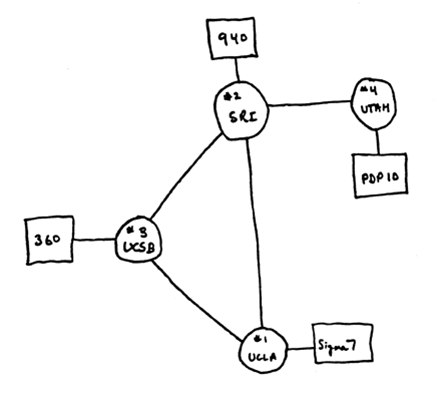
\includegraphics{figures/earlyarpanet}
    \caption{Early version of ARPANET \citep{website:computerhistory}} 
    \label{fig:earlyarpanet}
\end{figure}
\npar
After the first proof of concept ARPANET quickly expanded during the 1970s. It both expanded on the protocol it used and on the amount of connected nodes. We must first notice that in ARPANET there was no talk of client/server, it was originally designed as a peer-to-peer network \citep{petersalus2008, timbernerslee2000}. ARPANET also went outside the boundaries of the USA when it connected to a Norwegian node in 1973. Later other nodes were included such as a node in Britain, Sweden, \ldots (see image~\ref{fig:latearpanet}. The packet switching network left the proof-of-concept phase in 1975 when it was declared operational \citep{petersalus2008}. While the technology that ARPANET was run on is currently unimportant, the significance of the protocol that was used in this early network deemed to be humongous.  
\npar
When ARPANET was first launched in 1969 it used the 1822 protocol \citep{frankheart1970}, it was named after the report number. This protocol was designed to work cross-architecture and consisted of several fields: a message type, host address (numerical), and a data field. Messages were sent across the network using early routers, called: \emph{Interface Message Processors}. The entire system worked with either a direct, local link where messages were unicasted or were further broadcasted to other IMPs. Once the message had been successfully delivered and acknowledgment was sent back across the network to the sender. ARPANET was entirely designed for this protocol but on top of this protocol the NCP (Network Control Program) protocol was added which in essence meant that more layers were added. These protocols were deemed outdated in 1983 when the transition was made to TCP/IP. This caused a huge requirement of changes\footnote{Hence why this is one of the most notable \emph{flag days} in history of software}.
\npar
\begin{figure}[H]
    \centering
    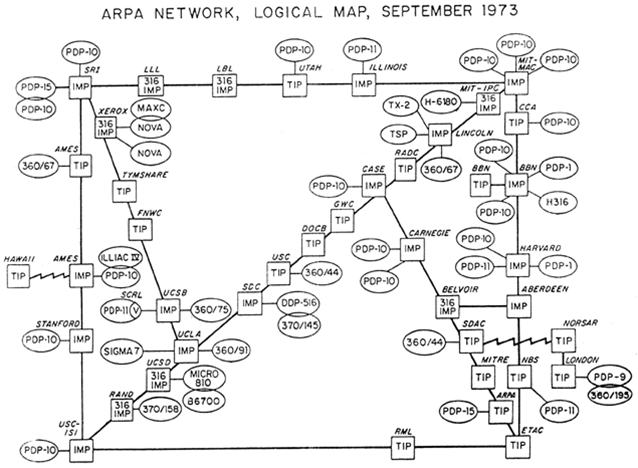
\includegraphics[width=0.8\textwidth]{figures/latearpanet}
    \caption{Late version of ARPANET \citep{website:computerhistory}} 
    \label{fig:latearpanet}
\end{figure}
\npar
In 1983 the transition was made towards the currently used TCP/IP protocol. This marked the start of the early \emph{Internet}. TCP/IP stands for Transport Control Protocol / Internet Protocol. This means it is in fact two protocols, transport layer protocol (TCP) and Internet Layer protocol (IP). ARPANET also allowed for layering of higher-level protocols and this is where the OSI model was born. ARPANET decommissioned in 1990 when the transition towards the current Internet had been made. This was mainly due the rise of ISPs (Internet Service Providers) in the late 1980s and 1990s. We can see that ARPANET was essential in the birth of the current Internet. 
\npar
In later years the Internet became a standardized product. Several standardization bodies regulate the current Internet. The one responsible for the TCP/IP standards is the Internet Engineering Task Force (IETF\footnote{\url{http://www.ietf.org/}}). While ISO (International Organization for Standards) is responsible for the overarching 7-layer model. Since the bottom part of the 5-layer model and the 7-layer model is exactly the same and we will be working close to the bottom, we will not be discussing the differences between these models further.


\subsection{Previous alternatives}

One of the most notable alternatives to ARPANET was the French-developed CYCLADES. It was created shortly after the birth of ARPANET. The main reason of this research project was to explore alternatives to ARPANET. The core principle was still the same though as also this network was a packet switching network. Some concepts from CYCLADES were later applied to the current version of the Internet, such as: host-responsibility and end-to-end protocol. 
\npar
At the time in the 1970s several research networks were developed. While all these networks were packet switching, the main point of argument was the role of network or host. Either the network or the host had to be responsible to deliver the packet and this divided the early networks in two groups. Other early research networks on packet switching were: DECnet, EIN nee COST II, EPSS, GEIS, IPX/SPX, Merit Network, \ldots. These networks were very similar to ARPANET and did not feature any noticeable new changes. The most important of these alternatives was CYCLADES and most of the flaws that ARPANET showed were filled by using technology and research from CYCLADES.

\subsection{Flaws of the current Internet}
\label{ssec:Internet_shortcomings}

The current model of Internet shows quite a few shortcomings. The main reason here is that the original protocols were never revised or alternatives were never considered. This static approach has lead to the use of a lot of hacks, patches, band-aids, \ldots. A very recent and obvious example is the need currently required to change from IPv4 towards IPv6. The reason for this is that we are simply running out of IPv4 addresses and thus we need another protocol to handle this. The question then rises: why do we need so many changes to a system that should be scalable? This questions can easily be answered when we look at the history of the Internet. It is based on a rigid system with very little science behind it. When we take a close look at the OSI model (see figure~\ref{fig:OSImodel}) we see a huge number of protocols who all have to work in conjunction with each other and overlap in several occasions\footnote{Example: IPv4 and IPv6 overlap}. 

\begin{figure}[H]
    \centering
    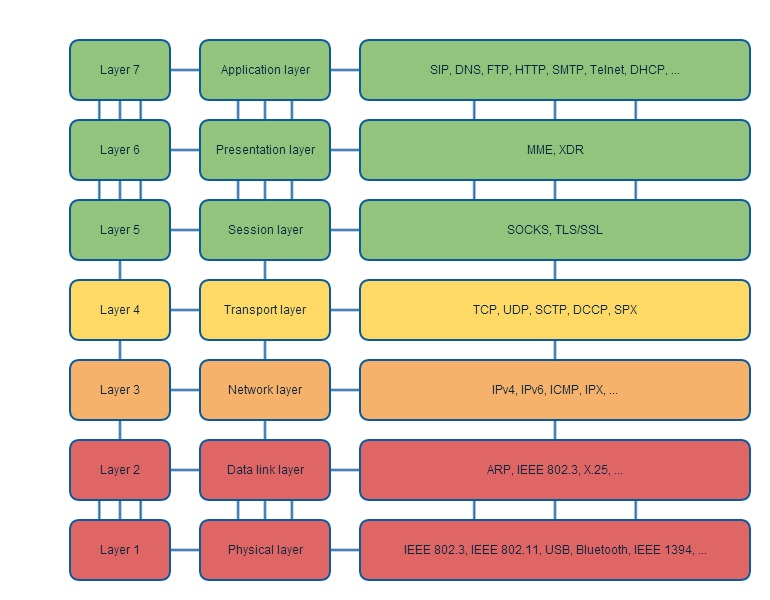
\includegraphics[width=\textwidth]{figures/osilayer}
    \caption{OSI model with examples} 
    \label{fig:OSImodel}
\end{figure}

\npar

Some examples of these issues in the current Internet are: multihoming, denial-of-service, port mapping, NAT (Network Address Translation), IP geomapping, \ldots. While some of these issues are solvable, they require a number of band-aids on the current Internet. This stems from the origin of the Internet. While it started out as a research net it was almost instantly made to be a production network. This was done while other networks, such as CYCLADES, were still researching and solving obvious problems. Due to faulty decisions the Internet continued to be build on these protocols and thus became flawed from the start. For example it is currently fairly difficult to send a packet with multihoming, this requires you to send two different packets. This also causes problems with mobility where targets change IP addresses quickly when running through different Internet providing cells. Handovers from routers is a big hassle for mobile users and slows down the entire process of staying online permanently. While short interruptions are not an issue when loading a website, it can prove fatal when using this Internet for live communications, monitoring, \ldots. Proper multihoming can potentially fix this issue, but this is currently very hard to achieve in the current state of the Internet. 
\npar
Another example is the use of NAT, Network Address Translation. This is needed because we are currently running out of IPv4 addresses and it enables small networks to have multiple nodes connected to the Internet at the same time. The problem is that this only solves issues in one direction. Nodes outside the network are in essence locked out of the network utilising NAT. While it might provide some basic safety benefits, it causes issues for several applications, such as peer-to-peer applications and many others. It also means that the router is actually breaching the model because it alters packets (specific port number and ip). In the normal model this is never changed between end hosts.
\npar
\begin{figure}[H]
    \centering
    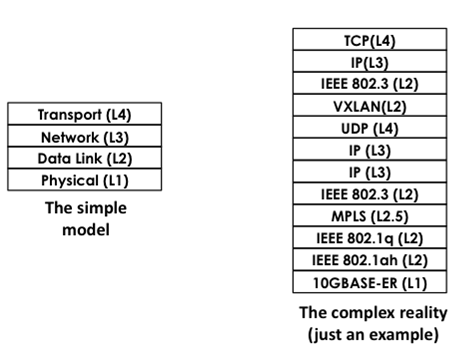
\includegraphics[width=0.9\textwidth]{figures/layeractualexamplenorina}
    \caption{Example of the current Internet layer system \citep{vrijders2014prototyping}} 
    \label{fig:layeractualexamplenorina}
\end{figure}
\npar
Further issues become apparent when looking at common items in some layers. We see that it is possible to map IP-addresses to geological information, thus violating privacy of the people using the Internet. Secondly when an attacker obtains an IP-address it becomes quite easy for this attacker to spam this IP with data causing a disruption in the service of the host. This is known as: Denial-of-Service Attack. Other mapping problems are the common application-port mapping that occurs. When anybody intercepts a packet he can read the port number and deduce for what application that packet can be used. This leads to more privacy issues and limits applications in their use as they are not free to choose a port number. 
\npar
We see that the current Internet has quite a lot of issues and can use a general, uniform model or architecture as an answer. Continuing down the road of constantly applying band-aids to a already broken system is clearly not an answer. A clear slate is needed and this is what the research question will try to find an answer for. 


\section{RINA alternative}
\label{sec:RINAalternative}
\epigraph{\emph{``Networking is Inter Process Communication (IPC) and IPC only''}}{John Day, \emph{Patterns in Network Architecture: A return to fundamentals}}

In this section we will address the alternative for the current Internet. This alternative is called \engels{Recursive InterNetworking Architecture} (RINA). We will start this section off with the main research question and state how this question will be answered. Following this we will take a closer look at RINA, both the function and the history will be discussed. The followup subsection will delve further into RINA and look towards the current technical implementation we are researching, \engels{Investigating RINA as Alternative to TCP/IP} (IRATI). After this section the reader is capable of comprehending how RINA functions and what the main research question is. 

\subsection{Research question}
\label{ssec:research_question}
We will first present the research question as this will clarify what will be researched, what should be developed and what answers we are looking for. This is applicable for both the literature study as well as for the entire thesis. 
\npar
The research question is stated as follows: \\
\begin{highlight}How to run RINA on Android over WiFi?\end{highlight}

\begin{figure}[H]
    \centering
    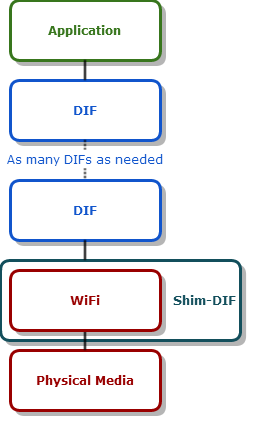
\includegraphics[width=0.4\textwidth]{figures/rinaoverwifi}
    \caption{RINA over WiFi} 
    \label{fig:rinaoverwifi}
\end{figure}
This is ultimately the question we are trying to answer. This question alone does not provide enough background and will need some further elaboration, which will be provided in this subsection. 
\npar
First we must note that RINA is the theory, actual working models are currently very scarce. We thus require a technical implementation of RINA. This will not be self constructed, we will be building further on a provided codebase. This project is \emph{Investigating RINA as Alternative to TCP/IP} (IRATI) \citep{vrijders2014prototyping}. This European project is a collaboration between: 
\begin{description}
	\item[i2CAT Foundation] \url{http://www.i2cat.net/en}
	\item[Nextworks] \url{http://www.nextworks.it}
	\item[iMinds] \url{http://www.iminds.be/en}
	\item[Interoute] \url{http://www.interoute.com/}
\end{description}
and is trying to bring a codebase for RINA upon which commercial implementations can be based. A working Recursive InterNetworking Architecture has already been developed for Linux operating systems. Since the Android platform is based on a trimmed and edited version of the Linux platform we will use the previously established code as a base. 
\npar

A current working Shim-DIF (more about specific working of RINA in \ref{ssec:RINAbasics}) has been constructed for 802.1Q (Ethernet) on Linux operating systems. A big portion of this research question is how to port the IRATI prototype on Android, more specifically to extend the prototype towards a working WiFi Shim-DIF. A key point for this Shim-DIF and the thesis as a whole is the need to be dependency free. When this Shim-DIF is dependency free it will guarantee the full and seamless working of RINA on mobile devices, specifically on the Android platform. Other physical connection mechanisms for Android such as: 3G, 4G, \ldots are not part of this thesis.
\npar
Another part of the research is dedicated towards the differences between the Linux and Android platform. Since IRATI is build in C in kernelspace and \cpp and Java in userspace.  These coding languages are well supported in Linux and in various other platforms. The issue here rises that the library that handles \cpp, \engels{glibc}, is not available in the Android operating system. On Android a variant of this library is available, called \engels{bionic}, this library however has more limited functionality, specifically some alterations on how \cpp is handled.
\npar
One final piece of research that will be completed is to figure out how to optimally map RINA API to the current WiFi standard. For this we will take a closer look at the current WiFi standard (802.11n) \citep{eldadperahia2008, sixtoortiz2009, thomaspaul2008}. We will examine the interaction this standard makes with several layers and where the Shim-DIF will some remodeling to seamlessly fit on the current WiFi standard.
\npar
This research question is now clearly stated and throughout this literature study we will try find the needed background information to help us formulate an answer in the thesis. The answer will not only be limited to pure text form, but shall also include working code for the prototype of the \emph{Shim-DIF over WiFi on Android}. 


\subsection{RINA basics and origin}
\label{ssec:RINAbasics}
Before we go any further we initiate with clearly stating what \engels{Recursive InterNetwork Architecture} (RINA) is, how it functions and what the origin of RINA is. As has been shown in subsection~\ref{ssec:Internet_shortcomings}, the current status of the Internet is facing a long list of issues. This is where RINA provides an adequate answer, it looks at previous network architectures and tries learn from those. In the end RINA proposes a basic, clear, and adequate answer for the networking needs.
\npar
RINA is a proposed architecture by John Day in his 2008 book: ``Patterns in Network Architecture: A return to fundamentals'' \citep{johnday2008}. 
Let us start by explaining the full name of RINA: \engels{Recursive InterNetwork Architecture}, first the last part: \engels{Architecture}, this states what the actual goal of this is. To implement an architecture that provides support for Network communication. One of the most important words in RINA is definitely: \engels{Recursive}. As can be seen in the IRATI symbol: a recursive tree. Recursive is defined as: ``pertaining to or using a rule or procedure that can be applied repeatedly.'' \citep{website:recursive_definition}, 
this instantly shows that the entire architecture is build on a base that can be repeated as many times as needed. It does not involve a static amount of layers, instead it can use as many or as few as needed to set up communication between two applications. The middle part: \engels{InterNetwork} shows that this architecture involves communication between and on networks and is not limited or restricted to single networks.
\npar
The main principle in RINA is that networking is simply and only: \engels{Inter-Process Communication} (IPC) \citep{johnday2008}. This is the premise on which entire RINA is founded on. An IPC is provided by IPC processes, a group of these coherent IPC processes forms a \engels{Distributed IPC Facility} (DIF) through enrollment. Every DIF is managed and has its own scope, it provides a way for processes to communicate between each other. DIFs have the same mechanism but are configured to different policies and thus have their own sets of rules. A DIF can ultimately be seen as a layer. For example the first DIF provides IPC directly to user applications. Below that you have a DIF that takes care of the communication between user A and the router user A is connected to. Every DIF has their own scope and once it becomes clear what the scope is for the DIF, the function of this DIF will be evident and be tailored to that scope. This repetition of DIFs goes on recursively until the entire chain of communication can be formed and finally the application from user A is interacting with the application from user B.
\npar
\begin{figure}[H]
    \centering
    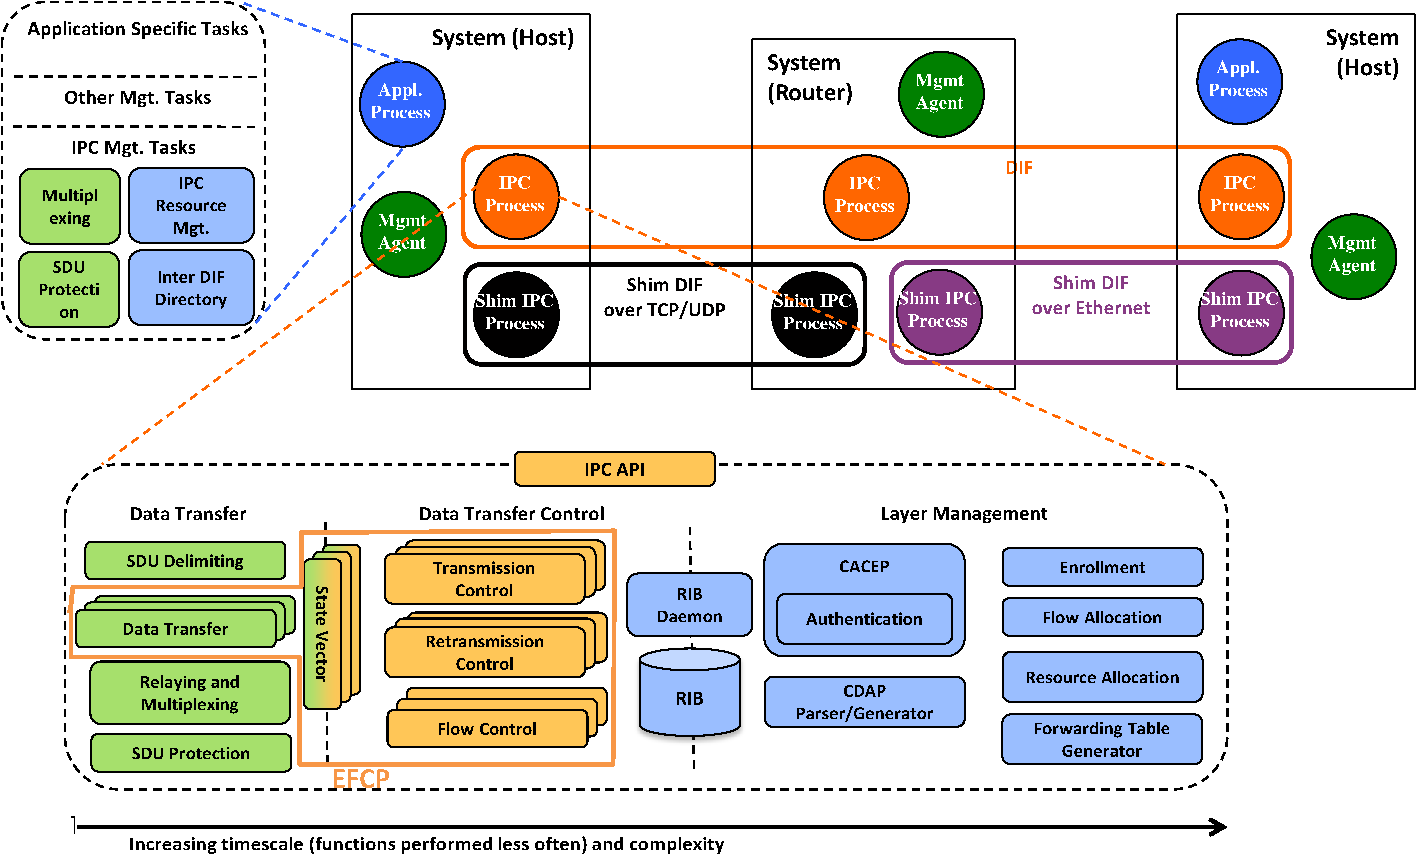
\includegraphics[width=\textwidth]{figures/referencemodel}
    \caption{Recursive InterNetworking Architecture example \citep{vrijders2014prototyping}} 
    \label{fig:RINAexample}
\end{figure}
\npar
An example how communication between two processes is established with RINA can be seen in the image~\ref{fig:RINAexample} above. Here we see application S on the host trying to communicate with application D on the other side of the communication chain. We see that for this specific example 3 levels of DIFs are used. These DIFs stack recursively from the bottom level (1st level) up till the DIF that actually takes care of the communication between the IPC and the application process. 
\npar
In this architecture we see that every application process, which also includes the IPC processes, has a name that is unique in that DIF. This is the way routing is ultimately done, but it no longer forces users to link applications to port numbers or specific IP addresses. While IP addresses can still be used in lower level DIFs for routing, the application does not to be aware of this. Naming stays within the DIF and is not visible outside that layer. In every DIF is a directory that contains these names of the IPC process names  and associates these to the application names (layer above the DIF). This is where we instantly see the possibility for multihoming. One application name can have different IPC processes in the layer below, but due to the design this application process does not need to be aware of this. The architecture will choose the most optimal routing and provide communication between the application processes in the layer above that requested it. Finally we must name the way a DIF sees it's surroundings. A DIF on the layer above is named the application. The process below the DIF is called the Point of Attachment. 


\subsection{IRATI implementation}

In this part we will address the technical implementation of the RINA model. The implementation that we will be using is developed in the IRATI project. 
\\
In this subsection we will further explain the current development status of IRATI, the future goals and give a brief explanation of the technical aspects of this project.
\npar
The IRATI project is building a working, open source, technical implementation of the Recursive InterNetwork Architecture in Linux with parts in both kernel and userspace\citep{website:IRATI-obj}. The technical roadmap towards this goal has been divided in 3 parts. 

\begin{enumerate}
	\item Restricted prototype (November 2013)
	\item Open source prototype (June 2014)
	\item Open source prototype, further development (December 2014)
\end{enumerate}

These different phases show the current plan of action for the project. They represent the coarse lines along which the project will guide itself. More specifically the project aims to have a technical implementation that features both parts in kernel space and in user space. These should be loosely coupled and functionalities that take part in both user and kernel space should be avoided. The reason that this currently has to be done is that for the entire architecture to work optimally we would need to have a brand new kernel based on this architecture. This is not within the confinement of the project and thus IRATI opts for a loosely coupled, although less optimal, system. Within this project is also a big part that represents the application programmable interface (API), this is fits itself within the user space. It acts as an adaptor in the project and presents the RINA stack towards the applications as a common interface. This is of utmost importance because thanks to this the applications quickly become versatile and cross platform. When the same API functions are offered on different platforms it becomes irrelevant for the application which operating system it is running on. As long as API functions presented to the the applications stay the same. This API currently offers bindings for C and \cpp for the applications. However bindings for other programming languages can be quickly implemented when using tools such as SWIG. SWIG stands for Simplified Wrapper and Interface Generator and can, when prompted present the C/\cpp bindings as other programming language bindings. A working example of this is the currently operational Java bindings for RINA. 

\npar

The first phase of the project focuses on having a working prototype of RINA. This prototype should be as low as possible within the current Internet stack. Due to not being able to fully redevelop a brand new kernel, outside the project's scope, the option has been made that the lowest feasible is the Ethernet stack. More specifically virtual LAN (vlan) Ethernet, 802.1Q. This requires one special DIF, a Shim-DIF over Ethernet that presents Ethernet in such a way that DIFs on top of this Shim-DIF can use it as part of RINA. This entire architecture is presented in the following figure~\ref{fig:rinaoverethernet}. This provides a technical proof-of-concept for RINA. It will also add functionality to current Internet, such as multihoming and improved mobility \citep{vrijders2014prototyping}. During this phase of the project the code is not publicly available.

\npar
\begin{figure}[H]
    \centering
    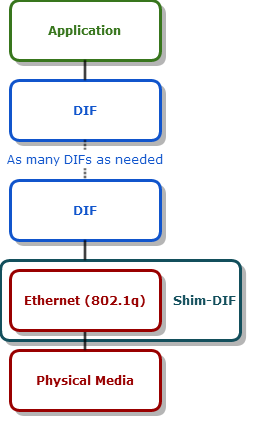
\includegraphics[width=0.4\textwidth]{figures/rinaoverethernet}
    \caption{Recursive InterNetworking Architecture example over Ethernet} 
    \label{fig:rinaoverethernet}
\end{figure}

\npar

After the first phase of the project has been completed and several iterations over the current code have been completed, it can move towards the open source phase. This should be around June 2014. In this phase functionality should be supplemented to the existing codebase. Not only should the previously working parts of the project be improved upon and publicly released, but new functionalities should be added. These items can be different levels of support on top of different layers of the current Internet. Expansions could be made towards other protocols than UDP or IP. Other platforms could be explored such as Android which is a minimal deviation from the current Linux Operating Systems that are being focused on. 

\npar
The final phase is to further iterate upon the currently existing codebase. This means fixing bugs and further improving functionality. These steps lead towards a well-developed technical project that clearly shows a proper implementation of RINA. During this phase further spread towards other operating systems and protocols is the main target. This will lead to a strong interoperability between different architectures and protocols using RINA. From the second phase on the project will be open sourced and aim to set up a strong developing community around the technical implementation of RINA. 

\npar

Finally we will briefly touch on how the thesis utilises the IRATI project. The thesis is focused on the WiFi implementation on Android operating systems (figure~\ref{fig:rinaoverwifi}). More specifically the thesis will aim to port the IRATI stack on the Android platform over WiFi. For this code will be used that was produced during the first phase. The code will be made publicly available when the second phase is reached, which should be at the end of this Master Thesis. 



\section{RINA on WiFi}

Following the introduction to the RINA alternative in section~\ref{sec:RINAalternative} we will now take a closer look to RINA over WiFi on Android. What the exact needs are for this implementation and where special focus will be needed. We kick this section off with a piece about IEEE 802.11 MAC protocol. Followed by the WiFi Shim-DIF. Finally we will take a closer look at the Android restrictions (compared to Linux).

\subsection{IEEE 802.11 Media Access Control}

In this subsection we will address the WiFi MAC\footnote{802.11 Media Access Control} \citep{matthewgast2005}. Since the protocol covers both layer 1 (physical layer) and a part of layer 2 (Media Access Control) we will limit ourselves here to the layer 2 interaction. The IRATI project code will have to fit seamless on this protocol to ensure maximal optimization for wireless communication. In this light we must instantly make an important remark. In normal operation mode the device drivers for user devices will be set to \emph{STA} mode (Station infrastructure mode). This enables basic device functions, however two devices in STA mode will not be able to communicate with each other unless an Access Point (AP) is presented to communicate with. As can been seen in figure~\ref{fig:80211inframode}.

\begin{figure}[H]
    \centering
    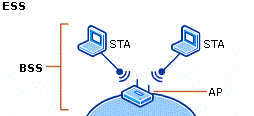
\includegraphics{figures/80211inframode}
    \caption{802.11 Infrastructure mode (STA and AP) \citep{website:80211microsoft}} 
    \label{fig:80211inframode}
\end{figure}

\npar

Drivers can also function in other modes, some of which will be handled later in this thesis, some who will not be handled at all. Other modes that drivers are capable of are \citep{website:80211wirelesskernel}: 
\begin{description}
	\item[AccessPoint (AP) infrastructure mode] Access Point for a master device in a network, normal mode for WiFi router. \emph{Not handled further}
	\item[Monitor (MON) mode] A passive mode that allows monitoring of all packets the device receives, can be double used in some devices. \emph{Used in testcases}
	\item[Ad-Hoc (IBSS) mode] Enables communication between other ad-hoc devices without AP (figure~\ref{fig:80211adhoc}). \emph{Used in testcases}

\begin{figure}[H]
    \centering
    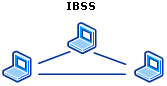
\includegraphics{figures/80211adhoc}
    \caption{802.11 Ad-hoc mode) \citep{website:80211microsoft}} 
    \label{fig:80211adhoc}
\end{figure}

	\item[Wireless Distribution System (WDS) mode] Enables communication between devices (mostly APs in a single ESS), uses the 4-addresses from the layer-2 header\footnote{Other modes only use these partially and mostly leave one or more fields empty}. \emph{Not handled further}
	\item[Mesh] Enables communication in Wireless Mesh Networks, used to set up intelligent, dynamic routes. \emph{Not handled further}
 \end{description}


\npar

For the initial part of this thesis we will leave the device in either STA or IBSS mode. This means that the drivers will \emph{translate} the 802.11 MAC-headers to 802.1Q MAC-headers when in STA mode. If this happens in IBSS mode we will have to test or ask authorized sources\footnote{Linux Wireless Kernel group for example}. The difference can be seen in the figure below (figure~\ref{fig:80211vs8021q}). We see that the entire header (Ethernet) becomes quite a bit easier to understand in STA mode. Since the IRATI project already has a working Ethernet Shim-DIF this will, under normal conditions, fit on this MAC header in STA mode. When expanding further down the road we will have to implement a Shim-DIF capable of handling the 802.11 MAC header. 


\begin{figure}[H]
    \centering
    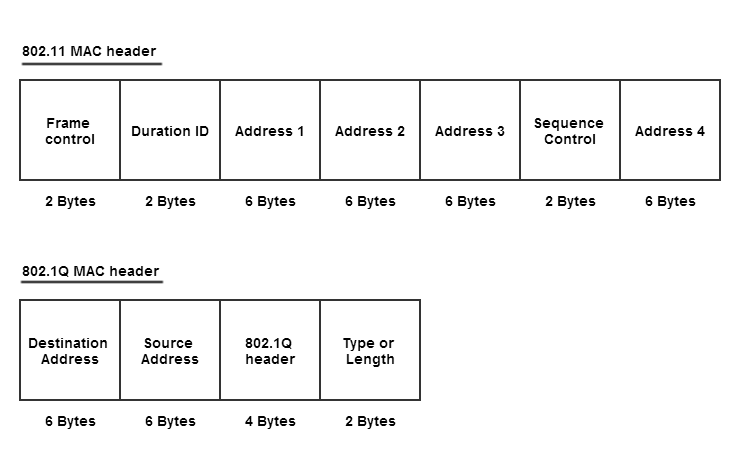
\includegraphics[width=0.8\textwidth]{figures/80211vs8021q}
    \caption{802.11 and 802.1Q MAC headers} 
    \label{fig:80211vs8021q}
\end{figure}

\npar

Since WiFi MAC headers (802.11 MAC) have quite a lot more functions (30 bytes compared to 802.1Q's 18 bytes) we will have to adjust the code for this. The functions that are added can potentially prove useful for the architecture and thus further study should be implemented. This research will focus on the overlap of functions between the MAC header and the functions provided by the IPC API. It can ultimately prove advantageous to use the full WiFI header alongside with RINA instead of having drivers reform this header to a more easy to comprehend Ethernet MAC header. 


\subsection{Shim-DIF for wireless}

While under normal operation of the research question we delve further into the Shim-DIF over WiFi (see figure~\ref{fig:rinaoverwifi}). However, due to reasons stated in the previous segment we clearly see that this has now been reformed to:

\begin{figure}[H]
    \centering
    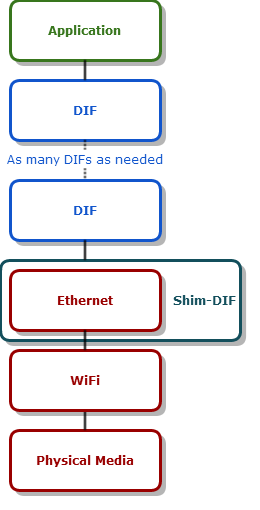
\includegraphics[width=0.4\textwidth]{figures/rinaoverwifi2}
    \caption{RINA over WiFi (updated)} 
    \label{fig:rinaoverwifi2}
\end{figure}

\npar
In normal conditions this means we can fully copy the code from IRATI, we must remind ourselves that we are still working on another Operating System and this comes with consequences. These are handled in the next component. We will take a closer look at the WiFi packets and provide a Shim-DIF for the WiFi standard. This provides a base for other developers who wish to update drivers further down to road to make said drivers compatible with RINA. 

\subsection{Android restrictions}

While Android is a UNIX-like operating system and based on Linux, it does come with some restrictions. In this subdivision we will be comparing Android OS to the Linux OS. The reason for this is that the IRATI project already has a working RINA implementation on Linux and this will be used for the further work of this thesis. Secondly because Android is based on Linux operating system and its kernel. At one point in history the two operating systems shared a common kernel and while this common component is planned, it is currently not the same kernel. 
\npar
Before we can further inspect the Android operating system, compared to Linux OS, we first need to identify the differences between the \emph{Android kernel} and \emph{Linux kernel}. For most of this information we will be using a talk by John Stultz, comparing Android to a stock Linux kernel \citep{presentation:android_linux_kernel,website:android_linux_kernel}. The amount of changes is not that large as it comprises of around 25 000 lines of changes, compared to the entire 15 millions lines of code for the full kernel. This places the changes around \textasciitilde0.2\% of the total code. Of course some of these changes can have large impacts on the actual kernel itself. These changes will be discussed here. Some of the items in the Android patches include:
\begin{itemize}
	\item Ashmem
	\item Binder
	\item Pmem
	\item Logger
	\item Early suspend
	\item Wakelocks
	\item Various small \emph{hacks} to facilitate a mobile OS
	\item \ldots
\end{itemize}
Because a Linux kernel is meant for desktop and server hardware (both very similar), Android aims to improve in the hardware department. This allows the use of more and varied hardware through its kernel. A second large point of interest for Android is the power management. While traditional systems are just plugged in with the cable and thus don't need to worry as much about power. The opposite is true for mobile, battery powered devices where power management is of utmost importance. Another change between the two kernels is the way error reporting is done and the attempt to increase security on the Android kernel. Finally the Android kernel aims to improve performance, especially for its intended users, mobile platforms.
\\
Some of these changes to the original kernel have been talked about quite a bit, such as the wakelocks. However we find that these changes will not impact the current implementation of the IRATI stack into Android. Further down the road additional optimization can be acquired between the Android kernel and the IRATI stack. Also RINA will have to be able to work with Paranoid Networking so that networking does not become blocked by this feature in Android kernels. For this part further research will be conducted. 
\npar
As shown above, the current version (and future versions) of the Android kernel will not pose any problems for the IRATI stack. However, an operating system does not only comprise of its kernel. This is an important part and the aspect where we see the biggest change between Linux and Android. When looking at a structured overview of an operating system (UNIX-like), we see that libraries play a big part in the undertaking of an operating system. Here we find the biggest change between Android and Linux. While Linux uses glibc \citep{website:glibc} and Android uses the Bionic library \citep{github:bionic,website:c_lib_bionic}. 
\npar
The restrictions from the Bionic library that affect the inclusion of the IRATI stack on Android are mostly limited to the \cpp language. The way Bionic handles \cpp is quite unique as it aims to alter the use of \cpp as a whole. This issue here is the following: IRATI stack is build on \cpp. For the most part \cpp is still supported by the library, but it does come with some restrictions. Before we inspect those restrictions we must first look at the reason why the glibc was not used in the first place. This can be declared very fast and accurate. Glibc is a \emph{slow} and \emph{huge} library. While this is not an issue for systems that run on Linux (desktops, servers, \ldots) it does form a problem for small-scale mobile platforms. Another issue with glibc is that it falls under GPL (GNU General Public License) and the smaller version, uClibC falls under LGPL (Lesser GNU General Public License). This implies that everything that uses these libraries also falls under these licenses, something Google was looking to avoid. Hence the option to use a new library, Bionic, which uses as BSD license and thus can shield its applications from the GPL and LGPL licenses. Finally we must note that glibc is quite large and meant for high frequency processors, where bionic is a lot smaller and works very fast, even without high speed processors\footnote{High frequency CPUs are becoming available for mobile platforms at this very moment}.
\npar
Because the \cpp restrictions of the Bionic library are of utmost importance to this IRATI project inclusion we will now take a closer look at these restrictions. The most profound and important restriction is the lack of support for \cpp exceptions. Google engineers deemed these exceptions bloated and largely impractical for use thus the support for this was entirely cut. When people still want to use exceptions they are advised to try another library, add a library that does support these or switch to Java programming language in the userspace. This is an important change as the current IRATI project does use \cpp exceptions and thus the code will need to be retailored to fit seamless on the Android platform. Another option is to try and implement changes on Android so that the current IRATI project can be ported over. Secondly, Bionic does not contain a \cpp Standard Template Library. This is for obvious reasons to try and keep Bionic as small as possible. When applications wish to use a \cpp STL they will have to include one with the application or acquire it beforehand. Other changes bionic made can be viewed at Pthreads. These are threads that are standardized and should be compatible cross-platform. Some changes bionic made to these threads include: cancellation, pthread\_once(), pthread\_atfork(). Here it is recommended that when these functions are used in the original code, to revise the code and work around these changes. The changes are in place again to reduce the bloated code in glibc and endorse optimized coding. The final changes that bionic implements are the lack of support for wide and locale characters and some user-account-related functions. 
\npar
Finally we see that the biggest restrictions on Android come from the use of the Bionic library. This library limits some uses of \cpp and requires a bypass from the original application. We note that the IRATI project is written partially in \cpp and uses exceptions. This will require a workaround on either the operating system side or on the IRATI project. How this will be handled is one of the major questions in this thesis. 


\section{Conclusion and placement of the study in the thesis}

In the final segment of this literature study we will draw a conclusion and show where the literature study will fit in the master thesis. The relevance of this entire literature study will be shown throughout the rest of thesis. It might become obsolete or perspectives might change, but this is a needed study. The study provides a baseline on which the Master's Thesis will build further. Several tests need to be conducted and code needs to be programmed, this means that the conclusion will be quite different. This also means that the literature study will be purely that and no conclusions will be drawn from only this aspect, the conclusions will be multi-faceted. 

\subsection{Conclusion literature study}

As we can see from the initial chapter the Internet is not perfect. It was built on a proof-of-concept with a very basic set of rigid protocols. This has lead to several disadvantages that currently require heaps of work for just temporarily repairs. For other issues we just require a plain new protocol to solve this issue. A clear answer is needed and this is what we present: Recursive InterNetworking Architecture, RINA. This new architecture requires quite a bit of initial work to set up a technical project to take over all the functions of the current Internet. After this initial work it will require minimal maintenance and prove to be very scalable in the long run. The main reason for this is the recursive function in the entire architecture.
\npar
RINA is an architecture that stands on one basic principle: networking is an InterProcess Communication (IPC) and IPC alone \citep{johnday2008}. This IPC is provides an IPC process. A group of these coherent processes (same layer) forms a Distributed IPC Facility (DIF) when these processes are enrolled. These DIFs stack recursively until the application on host A can communicate with the application on host B. Every one of these DIFs has a unique set of functions and operates in its own scope. 
\npar
This shows the way RINA functions, but since RINA is only a model we need a technical implementation. This implementation we will be using and supporting is the IRATI (Investigating RINA as Alternative to TCP/IP) project. This European project focuses on a technical implementation of RINA for UNIX-like operating systems. It already has a working Shim-DIF for Ethernet (802.1q). In this thesis we will try to port the IRATI stack to Android. Finally we will try to make a working Shim-DIF for WiFi on Android. 
\npar
Finally we take a closer look to the DIF that will be researched in this thesis. The Shim-DIF for wireless. This Shim-DIF will use the Ethernet MAC header as its main pillar and build further upon this. In research from this literature study we have concluded that 802.11 (WiFi) MAC headers are not available because drivers reform these to 802.3 headers. This means that the initial research question is altered in a manner that reflects these findings. To illustrate this with images: we initially started with image~\ref{fig:rinaoverwifi} and after this study we came to the conclusion that we will have to work on a model represented in image~\ref{fig:rinaoverwifi2}. When all the above questions have been answered and submitted, we can assume the research question (\ref{ssec:research_question}) has been solved.

\subsection{Placement of the literature study in the master thesis}

This literature study functions as a background study for the master thesis. In this study we have looked at the cause of the problem, clearly stated the research question, and finally we have provided adequate research to start the thesis. The background study and information has thus been provided to the researchers. This information shall be used to continue the thesis from this point on. Several research topics and points of importance have been pointed out in this study. 



\chapter{SHIM DIF for WiFi}

\section{Introduction}

In this chapter we will stipulate the Specification of the Shim DIF over WiFi. This DIF will only provide support for RINA DIFs. Given that a RINA DIF expects a RINA API as the lower API, the purpose of a Shim DIF is to create as thin a veneer as possible over a legacy protocol (WiFi) to allow a RINA DIF to use it without modification.  The goal is not to make legacy protocols provide full support for RINA and so the shim DIF should provide no more service or capability than the legacy protocol provides.

\npar

\begin{table}[H]
		\begin{center}
		\begin{tabular}{|lc|}
			\hline
				802.2 & LLC		\\ \hline
				802.11 & MAC		\\ \hline
				802.11 & PHY		\\
			\hline
		\end{tabular}
		\caption{Overview of WiFi protocol parts}
		\end{center}
\end{table}

WiFi consists of 3 main parts and the adaptor will try to span over all these. On top we have the 802.2 LLC layer, below that is the 802.11 MAC layer and finally we have the 802.11 physical layer. We must note that the LLC layer is an old protocol that has been reused for WiFi, it is not likely to be updated soon. The LLC layer is currently being used to differentiate between different higher level data packets. The MAC layer has been changed as recently as 2007 with 802.11e. It has several fields reserved for future use and could be changed later on. Finally, the physical layer is presented at the bottom of the WiFi scope. We instantly note that this changed quite often but provides no additional use towards the Shim DIF. The physical layer of WiFi is not within the scope of the Shim DIF. 

\npar

The Shim DIF over WiFi is not a fully functional DIF. This means that some limitations apply to this protocol:

\begin{itemize}
	\item Limited amount of flows due to the usage of the LLC header for flow differentiation (802.2 standard\citep{ieee8022std}).
	\item Only type 1 operation of LLC is useable, this means no Flow Allocation with LLC is possible.
\end{itemize}

The reason why we can only use Type 1 operation is because the other types (2 \& 3) require constant ACKing of packets. These packets are then marked with ACK numbers, limited to 128 different values. This is considered too low in the current high bandwidth traffic that can occur. Thus only Type 1 operation, which has no ACKing, but also Data State vectors, can be used. Even with these restrictions the Shim DIF provides enough support at the bottom layer of the architecture that other DIFs can build further upon. The Shim DIF provides QoS-cubes, flow differentiation and other options such as fragmentation possibilities. The Shim DIF presents the WiFi stack towards upper layer DIFs as a DIF.

\section{Mapping of 802.11 MAC header}

In this section we will show how we will use WiFi. We will start the mapping from the 802.11 MAC layer. Here we focus on 802.11e, this IEEE standard from 2005 implements the most recent version of MAC. This includes the introduction of QoS, used later on in this specification. 

\npar

The fields in the 802.11 MAC header (shown in figure~\ref{fig:80211macframe}) that will be used are the Address Fields and Payload field.

\begin{figure}[H]
    \centering
    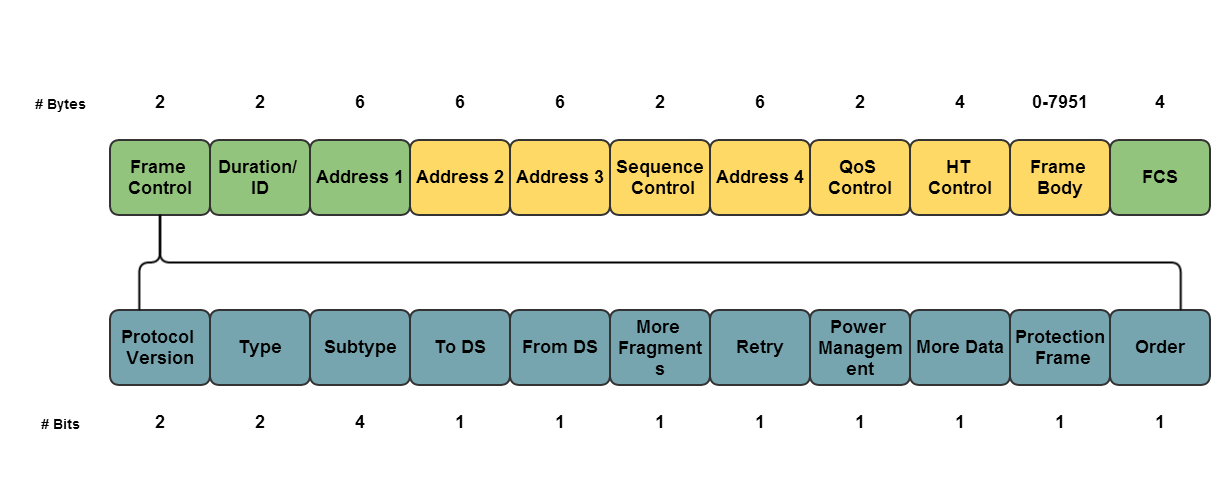
\includegraphics[width=1\textwidth]{figures/80211macframe}
    \caption{802.11 MAC frame} 
    \label{fig:80211macframe}
\end{figure}

These 4 address fields will be used according to the 802.11 MAC standard~\citep{ieee80211std}. This means the following address fields will be mapped:

\begin{description}

\item[Address fields] The MAC addresses used to identify shim IPC Processes to.
\\


%table for address fields
\begin{table}[H]
%\begin{adjustbox}{width=\textwidth,keepaspectratio}
	\begin{center}
		\begin{tabulary}{1.0\textwidth}{|L|L|L|L|L|L|L|}
			\hline
				\textbf{Network Type} & \textbf{To DS bit} & \textbf{From DS bit} & \nohyphens{\textbf{Address 1}} & \nohyphens{\textbf{Address 2}} & \nohyphens{\textbf{Address 3}} & \nohyphens{\textbf{Address 4}} \\ \hline
				IBSS (ad hoc) & 0 & 0 & DA & SA & BSSID & \emph{N/A} \\ \hline
				BSS (infrastructure) & 0 & 1 & DA & BSSID & SA & \emph{N/A} \\ \hline
				BSS (infrastructure) & 1 & 0 & BSSID & SA & DA & \emph{N/A} \\ \hline
				WDS & 1 & 1 & RA & TA & DA & SA \\
			\hline
		\end{tabulary}
		\caption[Overview of Address Fields]{Overview of Address Fields\protect\footnotemark}
	\end{center}
%\end{adjustbox}
\end{table}

\footnotetext{Only DA and SA are used in the Shim IPC Process}

%end table address fields
\begin{description}
	\item[Destination Address (DA)] The Shim IPC process address corresponding to the WiFi interface that the destination Shim IPC Process is bound to.
	\item[Source Address (SA)] The Shim IPC process address corresponding to the WiFi interface of this Shim IPC Process.
\end{description}

Note that these address fields are static in the Shim and are determined according to the values in the Frame Control field, further details shall not be provided for this as this is provided in the IEEE standard\citep{ieee80211std}.  

\item[Frame Body] This is the SDU it received from the upper DIF. An SDU can be fragmented as 802.11 supports fragmented payload\footnote{More Fragments subfield in the Frame Control field}

\end{description} 

The DIF name is the SSID (Service Set Identifier). This name is provided by periodical advertisement in a beacon frame.


\section{Mapping of 802.2 LLC header}

\begin{table}[H]
		\begin{center}
		\begin{tabular}{|c|c|c|c|}
			\hline
				\textbf{DSAP address} & \textbf{SSAP address} & \textbf{Control} & \textbf{Information} \\ \hline
				8 bits & 8 bits & 8 or 16 bits & M*8 bits \\ 
			\hline
		\end{tabular}
		\caption{802.2 LLC PDU format}
		\end{center}
\end{table}

The 802.2 LLC header will primarily be used for differentiating between different connections for the upper layer DIF. For further information and documentation on this standard we refer to the IEEE document~\citep{ieee8022std}.

\subsection{SAP addressing}
\label{ssec:sap-addressing}

SAPs will be used to distinguish between different connections, the current address assignments for SAP can be found in the table below. These SAP assignments only have to be unique within their scope and are not required to be globally unique. Every SAP is a CEP-id, during flow allocation they are mapped to a port-id. This port-id forms the boundary between the 0-DIF (Shim DIF) and the 1-DIF.

\npar

\begin{table}[H]
	\begin{center}
		\begin{tabular}{|c|c|c|c|c|c|c|c|c|c|c|c|c|c|c|c|}
			%\hline
				\multicolumn{8}{|l|}{$<$ Least significant bit} & \multicolumn{8}{l|}{$<$ Least significant bit} \\
				\hline
				I/G & D\textsuperscript{ISO} & D & D & D & D & D & D & C/R & S\textsuperscript{ISO} & S & S & S & S & S & S \\
				\hline
				\multicolumn{16}{l}{} \\
				\multicolumn{1}{l}{I/G} & \multicolumn{1}{l}{0} & \multicolumn{1}{l}{=} & \multicolumn{13}{l}{Individual DSAP} \\
				\multicolumn{1}{l}{I/G} & \multicolumn{1}{l}{1} & \multicolumn{1}{l}{=} & \multicolumn{13}{l}{Group DSAP} \\
				\multicolumn{1}{l}{C/R} & \multicolumn{1}{l}{0} & \multicolumn{1}{l}{=} & \multicolumn{13}{l}{Command} \\
				\multicolumn{1}{l}{C/R} & \multicolumn{1}{l}{1} & \multicolumn{1}{l}{=} & \multicolumn{13}{l}{Response} \\
				\multicolumn{1}{l}{I/G} &  \multicolumn{2}{l}{\texttt{0 DD DDDD}} & \multicolumn{1}{l}{=} & \multicolumn{12}{l}{DSAP address} \\
				\multicolumn{1}{l}{C/R} &  \multicolumn{2}{l}{\texttt{0 SS SSSS}} & \multicolumn{1}{l}{=} & \multicolumn{12}{l}{SSAP address} \\
				\multicolumn{1}{l}{I/G} &  \multicolumn{2}{l}{\texttt{1 DD DDDD}} & \multicolumn{1}{l}{=} & \multicolumn{12}{l}{Reserved for ISO definition} \\
				\multicolumn{1}{l}{C/R} &  \multicolumn{2}{l}{\texttt{1 SS SSSS}} & \multicolumn{1}{l}{=} & \multicolumn{12}{l}{Reserved for ISO definition} \\
				
				
			%\hline
		\end{tabular}
		\caption{SAP Address Assignment}
	\end{center}
\end{table}

\npar

This leaves 6 bits per address field free to choose. The least significant bit is always on the left. We will only use individual SAPs and discard the Command/Response bit due to not having Data State Vectors available. The second least significant bit will also be left 0, due to the ISO definition. This means we can only use \{0, 4, 8, C\} for our last hex symbol. This leaves the following possibilities free to choose from: 0x\{XY\}. With X = \{0, 1, 2, 3, 4, 5, 6, 7, 8, 9, A, B, C, D, E, F\} and Y = \{0, 4, 8, C\}. In total, 64 SAP addresses can be used within the Shim DIF.



\subsection{DSAP address field}

The Destination Service Access Point will be used to identify the flow on the destination IPC Process. For correct mapping on addressing we currently store a mapping between application-naming and connection address locally.

\subsection{SSAP address field}

The Source Service Access Point will be used for to identify the flow on the current IPC Process. For correct mapping on addressing we currently store a mapping between application-naming and connection address locally.

\section{Use of Address Resolution Protocol}
\label{sec:arp}

Because the RINA Flow Allocator is unavailable at this low level, the Shim DIF reuses ARP in a request/response mode to perform Flow Allocation. ARP \citep{arp1998} will be used to map an application-naming (1-DIF) to the address of a Shim IPC Process (0-DIF). Currently ARP is used to map a hardware address to an IP(v4) address. 
\\
Below is the ARP frame represented by  the RFC826 implementation\footnote{\url{http://tools.ietf.org/html/rfc826}}. 


\begin{table}[H]
	\begin{center}
		\begin{tabular}{|c|c|}
			\hline
				\textbf{Bit 0-7} & \textbf{Bit 8-15} \\ \hline
				\multicolumn{2}{|c|}{Hardware type} \\ \hline
				\multicolumn{2}{|c|}{Protocol ethertype} \\ \hline
				Hardware address byte length & Protocol address byte length \\ \hline
				\multicolumn{2}{|c|}{Opcode (ARP Request or ARP Response)} \\ \hline
				\multicolumn{2}{|c|}{Hardware address sender (n bytes)} \\ \hline
				\multicolumn{2}{|c|}{Protocol address sender (m bytes)} \\ \hline
				\multicolumn{2}{|c|}{Hardware address target (if known) (n bytes)} \\ \hline
				\multicolumn{2}{|c|}{Protocol address target (m bytes)} \\ \hline
		\end{tabular}
		\caption{ARP frame format}
	\end{center}
\end{table}

\npar

In the chart below we show how ARP is used in the Shim DIF. Locally an ARP table is kept with entries which map Shim IPC Process Addresses (MAC addresses) to Application names. When data transfer is required, the Shim IPC Process asks the ARP protocol to send out an ARP request to find the Shim IPC Process Address which corresponds to the application name of the destination. 

\npar

\begin{figure}[H]
    \centering
    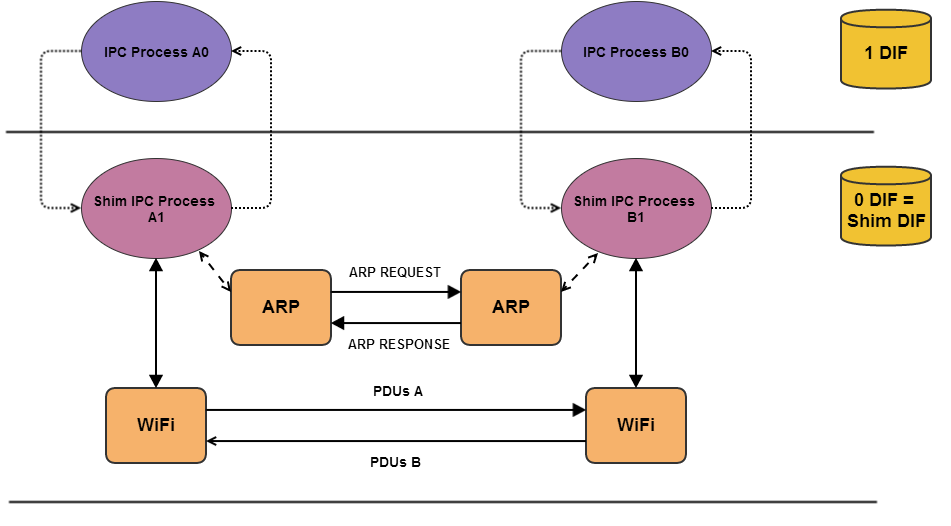
\includegraphics[width=1\textwidth]{figures/arp_example}
    \caption{ARP example} 
    \label{fig:arp_example}
\end{figure}

\npar

ARP has a 1 byte length field for the network protocol address. For the Shim DIF we will be using ASCII coding, this leaves us with a maximum of 255 characters for the length of the network protocol address. Due to RINA specifications, a name can consist of 4 parts, which will be encoded in this network protocol address. The encoding we use is bencoding. It is defined in the specification\footnote{\url{https://wiki.theory.org/BitTorrentSpecification\#Bencoding}} with the bittorrent protocol.

\npar

\begin{table}[H]
	\begin{center}
		\begin{tabular}{|l|l|}
			\hline
				Process name & Echo-IPC-Process  \\ \hline
				Process instance & 1 \\ \hline
				Entity name & Data \\ \hline
				Entity instance & 1 \\ \hline
		\end{tabular}
		\caption{Application-Naming information}
	\end{center}
\end{table}

\npar

Encoded this becomes: ``16:Echo-IPC-Process1:14:Data1:1''. Note that these are all strings. As an alternative we can also use a synonym for the application name. A synonym is the name of the Application Process instance with a default Application Entity instance. 
\\
Since we need to send the source and destination application name, but we only have one network protocol length field, we choose the longest application name. The other, shorter application name is then filled with padding (zero bytes, 0x00) which are removed by the receiving IPC Process. This causes some overhead, but this overhead stays very small because these ARP frames only need to be sent during the flow allocation phase.


\section{Service Definition}

In this section the different QoS-cubes that are supported will be addressed.

\subsection{QoS-cubes supported}

The WiFi protocol supports several QoS-cubes, they are a combination of following possibilities. 
\npar
Because QoS-cubes are separated in 4 categories we will offer 4 QoS-cubes. The categories are the following: voice, video, background, best effort. This gives us the following QoS cubes:

\begin{table}[H]
		\begin{center}
		\begin{tabular}{|l|l|}
			\hline
				ID 										& 		1 \\ \hline
				Name 									&			Voice \\ \hline
				Average bandwidth 		&			Depends on 802.11 physical standard \\ \hline
				Average SDU bandwidth 									&			Depends on 802.11 physical standard										 \\ \hline
				Peak bandwidth-duration 									&		Depends on 802.11 physical standard											 \\ \hline
				Peak SDU bandwidth-duration 									&			Depends on 802.11 physical standard										 \\ \hline
				Burst period 									&			Depends on 802.11 physical standard										 \\ \hline
				Burst duration 									&		Depends on 802.11 physical standard											 \\ \hline
				Undetected bit error rate 									&			Depends on 802.11 physical standard										 \\ \hline
				Partial delivery 									&			Allowed										 \\ \hline
				Order 									&				Depends on 802.11 physical standard									 \\ \hline
				Max allowable gap in SDUs 				&				Depends on 802.11 physical standard									 \\ \hline
				Delay 									&			Depends on 802-11 physical	standard									 \\ \hline
				Jitter 									&			Depends on 802-11 physical standard										 \\ \hline
				Ack policy							&			Depends on kernel settings				\\ \hline
		\end{tabular}
		\caption{QoS cube for traffic categorized as Voice}
		\end{center}
\end{table}

\npar

\begin{table}[H]
	\begin{center}
		\begin{tabular}{|l|l|}
			\hline
				ID & 2  \\ \hline
				Name & Video \\ \hline
		\end{tabular}
		\caption{QoS cube for traffic categorized as Video}
	\end{center}
\end{table}

\npar

\begin{table}[H]
	\begin{center}
		\begin{tabular}{|l|l|}
			\hline
				ID & 3  \\ \hline
				Name & Background \\ \hline
		\end{tabular}
		\caption{QoS cube for traffic categorized as Background}
	\end{center}
\end{table}

\npar

\begin{table}[H]
	\begin{center}
		\begin{tabular}{|l|l|}
			\hline
				ID & 4  \\ \hline
				Name & Best\_effort  \\ \hline
		\end{tabular}
		\caption{QoS cube for traffic categorized as Best effort}
	\end{center}
\end{table}

Note that we do not provide full tables as below the Name section these are all the same, dependent on the physical standard over which communication is done. 

\section{Configuration}

Every Shim IPC Process is assigned to a WiFi interface. Before the Shim DIF can become operational it needs a basic amount of information. This information is comprised of:

\subsection{Shim IPC Process info}

The Shim IPC Process needs information on the device to which it is bound. This information is: name of device (wlan0, \ldots), hardware address of the device, state of the device (UP/DOWN). Furthermore it requires information to interact with the wireless network this device is part of. This information consists of: SSID, Encryption, Channel, Encryption-key.

\subsection{Port-id to CEP-id directory}

The WiFi Shim DIF has different flows available through the use of CEP-ids. In the subsection~\ref{ssec:sap-addressing} about SAP mapping we saw that 64 connections can be differentiated. Each one has a 1-byte long address. This SAP address is a Connection EndPoint-Identifier (CEP-id). The CEP-id is locally mapped on the port-id. The port-id is a transfer point on the boundary between the 1-DIF and the 0-DIF. 

\subsection{Application to SAP mapping}

Since no explicit flow allocation is possible, it is currently not possible to choose the SAP addresses freely. They will be mapped to applications locally in a file. This file contains a mapping for application naming info to SAP addresses. When communication is set up the Shim IPC Process retrieves the right SAP address from this file based on the requesting application. Or the Shim IPC Process delivers to the correct application process based on the SAP address. 

\section{Bootstrapping}

Upon creation of the Shim IPC Process, the Shim IPC Process assumes its position in the DIF. This DIF name is the same name as the SSID. First the Shim IPC process is bound to the interface and assumes the Shim IPC Process address is the same as the hardware address of the wireless device. When this wireless device becomes part of the network, the Shim IPC Process is considered to be part of the DIF. When these conditions have been met, we assume that all traffic will be RINA traffic and should be handled by the Shim DIF.

\section{Application (un)registration}

If an Application Process (AP) registers with the Shim IPC Process. Upon registration of the application, the Shim IPC Process's directory adds an item. This item maps the AP name to the MAC address. The MAC address is bound to the Shim IPC process. Finally when an AP un-registers the Shim IPC Process removes the entry in the ARP cache. If future queries of the application name are triggered, they will be ignored if the entry is not present in the cache.

\section{Enrollment}

All members with an interface active in the same SSID are assumed to be in the same Shim DIF. When a new member enlists in this Service Set it is enrolled in the Shim DIF. 

\section{WiFi Shim IPC Process Definition}
\label{sec:wifi_shim_ipc_proc_def}

The Shim IPC process over WiFi assumes the following API from ARP:

\begin{description}
	\item[arpAdd(netaddress).submit] Adds a mapping of network address, in RINA the application name, to the MAC interface in the ARP table of the interface. In essence this maps the application process to the Shim IPC process address. The function returns: 'success' when the mapping was added, 'failure' when it was not. 
	\item[arpRemove(netaddress).submit] This is the inverse of the action of the previous function. It removes a mapping of the application name to the MAC address in the ARP table. If this entry is removed it returns: 'success', otherwise 'failure' is returned.
	\item[arpMapping(netaddress).submit] Requests ARP for a mapping of a network address to a MAC address. When the mapping is found, arpMapping(netaddress, hwaddress).deliver is called.
\end{description}

These 3 functions are provided by ARP.

	 

\npar

Port-ids are linked to CEP-ids and are tristate variables. The 3 states of a port-id are the following:

\begin{description}
	\item[NULL] The port-id is unusable in this state
	\item[PENDING-SAP] This state of the port-id can originate from two possibilities. The application process has initiated the flow allocation, requested sapMapping and is idle in the PENDING-SAP state until it receives an sapMapping.deliver. The other option is that it has received a request to create a flow and is currently waiting for the sapMapping.submit function to finish, it stays in the PENDING-SAP until it receives sapMapping.deliver.
	\item[PENDING-ARP] This state of the port-id can originate from 2 possibilities. The port-id has received the sapMapping.deliver(+) function and the arpMapping.query has been called. The port is idle in the PENDING-ARP state until it receives the arpMapping.deliver. The other possibility is that the request to create a flow has delivered the sapMapping.deliver(+) and is waiting for the allocateResponse.submit to finish the flow allocation.
	\item[ALLOCATED] This state indicates that the flow has been allocated and the port-id can be used to read/write data to/from.
\end{description}

\npar

Below are all the possible functions for the Shim IPC process and finally a state diagram with said functions is presented.

\subsection{applicationRegister(naming-info).submit}
\subsubsection{When invoked}
This primitive is invoked to register an application on top of the shim IPC process.  The application becomes available in the shim DIF. This primitive has to be invoked before all other functions. ARP does not differentiate between client/server, which means every application has to be available in the ARP table, even clients.
\subsubsection{Action upon receipt}
The naming-info is transformed into a single string (application-name), with the method described in segment~\ref{sec:arp}. arpAdd(application-name).submit is called. If successful, a mapping of the application name to the hardware address of the device is added in the ARP table of the interface. The other primitives become usable. If it failed, they are not and an error is generated.


\subsection{applicationUnregister(naming-info).submit}
\subsubsection{When invoked}
This primitive is invoked to unregister an application on top of the shim IPC process. This unregisters the application in the shim DIF. No other primitives can be invoked until applicationRegister(naming-info).submit is called again. 
\subsubsection{Action upon receipt}
The naming-info is transformed into a single string (application-name), with the method described in section~\ref{sec:arp}. arpRemove(application-name).submit is called. If successful, the mapping of the application name to the hardware address of the device is removed from the ARP table of the device. If it fails, an error is generated.


\subsection{allocateRequest(naming-info).submit}
\subsubsection{When invoked}
This primitive is invoked by a source application to request a new flow. Naming-info consists of the destination upper layer IPC Process name $<$AP name, AE name$>$ (AP-name if there is a single Shim-DIF; AP-ApplicationEntity if there is more than one).
\subsubsection{Action upon receipt}
If there is already a flow established to the destination application (the port-id is in the ALLOCATED state), or there is a flow pending between the source and destination applications (the port-id is in the PENDING-SAP or PENDING-ARP state), a negative allocateResponse(reason).deliver is returned. If the port-id is in the NULL state, sapMapping(void, port-id,netaddr).submit is called. The port-id transitions to the PENDING-SAP state.


\subsection{allocateResponse(reason).submit}
\subsubsection{When invoked}
This primitive is invoked by the destination application in response to an allocateRequest(naming-info).deliver which is invoked by a positive sapMapping(reason).deliver.
\subsubsection{Action upon receipt}
If the port-id is not in the PENDING-ARP state, an error is generated. If it is and if the allocate response is positive a flow has been established for this port-id; any queued frames are delivered to the destination application. The port-id transitions to the ALLOCATED state. If it is negative the flow creation has failed and reason indicates the failure reason, all queued and future frames from this combination of source MAC address and source SAP are dropped. The port-id transitions to the NULL state.


\subsection{arpMapping(netaddr,hwaddr).deliver}
\subsubsection{When invoked}
This is invoked by the ARP protocol machine when a requested mapping becomes available in the ARP table. The Shim IPC process is supplied with the mapping of a network protocol address, application name in RINA, to a hardware address (hwaddr).
\subsubsection{Action upon receipt}
If the port-id is in the PENDING state, (there is an outstanding allocateRequest(naming-info).submit), an allocateResponse(reason).deliver is invoked, and the hardware address (MAC address) is stored for this flow.  In this case the port-id transitions to the ALLOCATED state. If the port-id is in the ALLOCATED state, nothing happens. If it is in any other state, an error is generated.

\subsection{sapMapping(CEP-id,Port-id,Naming-info).query}
\subsubsection{When invoked}
This can be invoked by the reception of a WiFi frame when the port-id is in the NULL state. The port-id transitions to the PENDING-SAP state and the Shim IPC process awaits the sapMapping(reason).deliver response. It can also be invoked by the allocateRequest.submit function. The port-id transitions to the PENDING-SAP state and awaits the sapMapping(reason).deliver response. If the port is in the ALLOCATED nothing happens.
\subsubsection{Action upon receipt}
When received, the locally stored ``SAP to naming-information'' database is queried. The response is the sapMapping(reason).deliver response.

\subsection{sapMapping(CEP-id,Port-id,Application-naming).submit}
\subsubsection{When invoked}
When a mapping is found by sapMapping(CEP-id,Port-id,Naming-info) this function is invoked.
\subsubsection{Action upon receipt} 
Requests the Shim IPC Process to look in the provided table to find a mapping between the CEP-id and the Application-naming. If successful this adds an entry to the ``Port-id to CEP-id directory'' and consequently calls a positive sapMapping.deliver(+). If the unsuccessful a negative sapMapping.deliver(-) is called and no mapping is added to the CEP-id to Port-id directory. Note that this function always requires a Port-id and either a CEP-id (receiving Shim IPC Process) or Application-naming (sending Shim IPC Process). 

\subsection{sapMapping(reason).deliver}
\subsubsection{When invoked}
This is invoked as a response to the sapMapping(CEP-id,Port-id,Naming-info).query after the ``SAP to naming-information'' has been inquired. 
\subsubsection{Action upon receipt}
If the naming-info is an error (sapMapping.deliver(-)) then the port-id transitions to the NULL state. If the information is genuine and the port-id was in the PENDING-SAP state then it transitions to the PENDING-ARP state. 

\subsection{Frame}
\subsubsection{When invoked}
When the port-id is in the ALLOCATED state, a frame may be sent.  Otherwise the frame is dropped.
\subsubsection{Action upon receipt}
When there is no flow for the combination of the MAC address that sent the frame and the receiving CEP-id, the sapMapping.query function is called and the port-id transitions to PENDING-SAP. If there is a flow for the sender's MAC address and the receiving CEP-id, and the port-id is in the ALLOCATED state, write.deliver is called. If it is in the PENDING-SAP or PENDING-ARP state, the packet is queued. If it is in the NULL state, the packet is dropped.


\subsection{read.submit}
\subsubsection{When invoked}
This is invoked by the application when it wants to read a SDU.
\subsubsection{Action upon receipt}
When the shim IPC process receives this primitive and the port-id is in the ALLOCATED state, it will create a frame, and pass it to the OS for delivery. It is assumed that neither fragmentation nor concatenation is performed by the shim IPC Process. This is done because the WiFi protocol provides the functions below the Shim-DIF. Therefore shim IPC Process uses a different frame for each SDU passed to it. If the port-id is not in the ALLOCATED state, an error is generated and the frame is dropped.


\subsection{write.submit}
\subsubsection{When invoked}
This is invoked by the application when it wants to send one or more SDUs. 
\subsubsection{Action upon receipt}
When the shim IPC process receives this primitive and the port-id is in the ALLOCATED state, it will create a frame, and pass it to the OS for delivery. It is assumed that neither fragmentation nor concatenation is performed by the shim IPC Process. This is done because the WiFi protocol provides the functions below the Shim-DIF. Therefore shim IPC Process uses a different frame for each SDU passed to it. If the port-id is not in the ALLOCATED state, an error is generated and the frame is dropped. 


\subsection{deallocate.submit}
\subsubsection{When invoked}
This service primitive is invoked by the application to discard all state regarding this flow. It is the responsibility of both the source and destination application to invoke this primitive. It is a local event.
\subsubsection{Action upon receipt}
When the shim IPC process receives this primitive, the port-id transitions to the NULL state.


\subsection{Corresponding state diagram}

A ``/'' represents a following, or void, function that is being called by the preceding function. 

\begin{figure}[H]
    \centering
    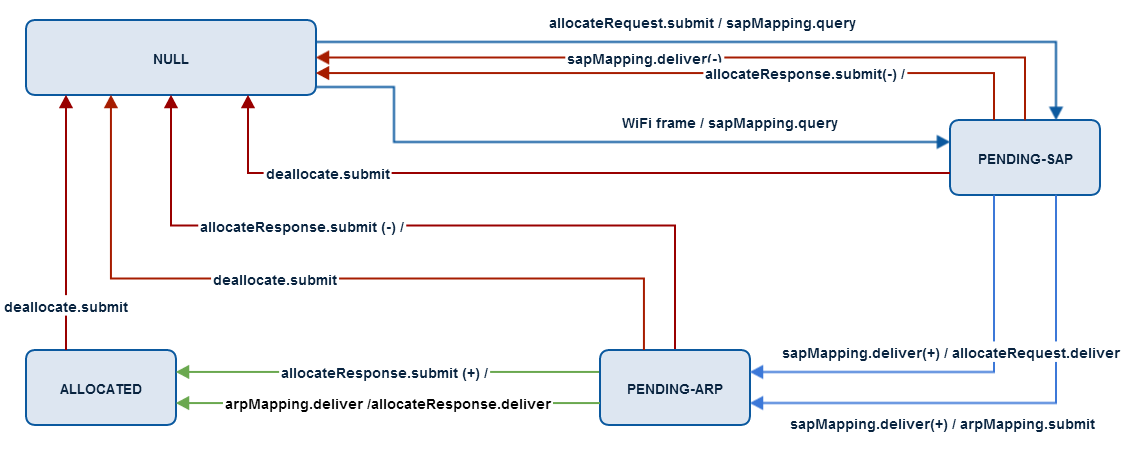
\includegraphics[height=0.6\textwidth, angle=270]{figures/state_diagram2}
    \caption{Corresponding state diagram} 
    \label{fig:state_diagram}
\end{figure}


\chapter{Implementation}

Ensuing the chapter about the specification over WiFi, we will now address the implementation of the prototype. This chapter has been divided in 3 sections, each containing a number of subsections. We initiate with the plan of action which clearly states the trajectory this implementation will follow. Secondly we focus on the implementation of a Shim DIF prototype over WiFi. Finally we approach the subject of the Android implementation. 

\section{Plan of action}

%Section detailing the course that will be followed through this chapter. This shows a guide for the reader which allows the reader to understand the different steps taken in the implementation.

In this section we will give the reader a short introduction to the implementation topic. After this introduction we have the procedure of implementation. This subsection will detail the path followed for this entire implementation and will clearly show the milestones on the path. The section can be seen as a guide to understand the different steps taken in the implementation part. 

\subsection{Introduction}

%Quick introduction to reiterate the research question and how this implementation will try to help to answer it

The research question states: ``How to run RINA on Android over WiFi?''. Now that the background of this question has been clearly evaluated we can move towards the implementation. This chapter seeks to find a way towards a technical implementation of this research question. The chapter will not instantly address the question, but will start with some basic proof of concepts and already working implementations. After these have been carefully explained on how they were achieved, we move further towards the WiFi part of the research question and finally altering the operating system (OS) to Android. 
\npar
In the end we hope to have a working, technical implementation of the IRATI project code that can be constructed and applied to the given test devices\footnote{Test devices = 2x Samsung Galaxy S II smartphones}.

\subsection{Procedure of implementation}

%Define the exact procedure that will be followed of the implementation. Starting with setting up test bench with first 2 virtual devices that run the test provided by IRATI. Then try proof of concept over WiFi, if needed with two physical notebooks, if possible, install wifi device virtual and implement virtual again. After this is done, brief explanation on how to compile android kernel with glibc. Then the android kernel with glibc and the irati stack. Final steps involve the installation of this kernel on the target devices. 

In the final part of this section we will discuss in detail how the implementation will be addressed. For this, we reference to figure~\ref{fig:poi-flowchart}. This figure shows us clearly all the steps that will be talked about in this chapter. The steps with higher importance to this thesis will be specified and will be addressed in greater detail. 

\npar

\begin{figure}[H]
    \centering
    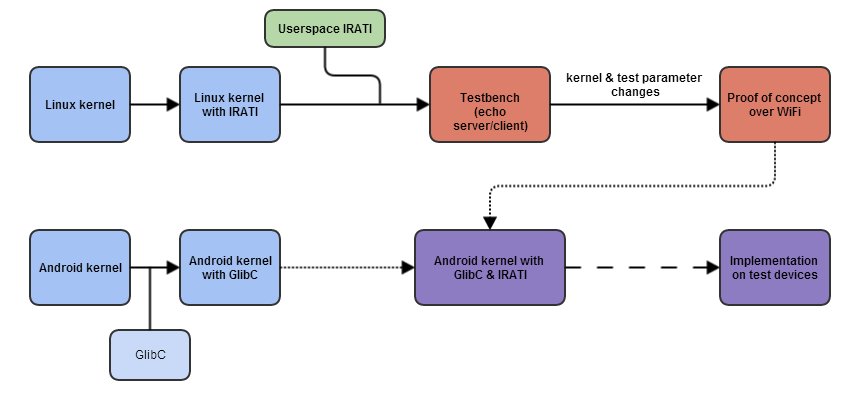
\includegraphics[width=1\textwidth]{figures/procedureofimplementation}
    \caption{Procedure of implementation - flow chart} 
    \label{fig:poi-flowchart}
\end{figure}

\npar

First we start with a proof of concept over WiFi. For this we use 2 linux machines who communicate through a simple echo program using RINA. This is an initial proof of concept that is needed to prove the capability of using RINA on top of WiFi. The point is here to prove that even though the WiFi frames are reformed to Ethernet frames by the drivers we can use these Ethernet frames for RINA. This is done by adding a VLAN interface (802.1Q) and using the Ethernet Shim DIF on top of this. This Ethernet Shim DIF and its functions are provided by the IRATI project. 
\\
The section initiates with an explanation on kernel compilation, where we briefly touch on how to build and install kernels. This a very basic step in the implementation that will see further use throughout the rest of the implementation chapter. Following this we prove the functionality of the Ethernet Shim DIF by setting up two virtual machines with RINA-enabled kernels that have the Ethernet Shim DIF. These are basic linux kernels with additions from the IRATI project. Finally we realize the proof of concept over WiFi. For this we use the linux kernels with both RINA and the IRATI additions enabled, plus the wireless parts added. 


\npar
After we have implemented a working RINA on pure linux machines, we initialize the process again on Android. We first note that also in Android the WiFi frames are transformed to Ethernet frames and only after this has been handled the user can use these frames. Specifically this means that once the kernel has been sufficiently modified for functionality on Android, that the wireless part is in essence the same as on pure linux computers. 
\\
Initially we explain how to build a basic android kernel and the differences to building a pure linux kernel. Secondly we explain how the IRATI-specific kernel parts are added to this base Android kernel. After this step we move towards adding the userspace implementation of the IRATI project. Because of previously mentioned limitation we require certain libraries so the addition of  glibc or a similar library will be required. Following this, we explain how the required userspace packages are added and how the userspace is configured. Once we are able to insert the modules and turn on the ipcmanager we can call this implementation a success. For the final part we explain the changes required to move from this basic Android kernel to a device specific kernel and run the echo experiment on the two test devices. 
\npar
We provide steps along this route on how we got to these parts, why we chose certain items over their respective alternatives and finally provide initial results to prove the functioning aspects of these implementations. 


\section{Proof of concept over WiFi}

In this section we will explain the implementation of the proof of concept of RINA over WiFi. This includes the compilation of a Linux kernel, the irati test bench setup and finally we show the proof of concept. 

\subsection{Compiling a kernel}

The first step of the implementation is building a base kernel. For this step we have several possibilities and guides available. While we will not go into details such as listing exact commands we intend to give a clear structure on how to build a basic kernel for a Linux Operating System. The reason we choose Linux is fairly straightforward:

\begin{itemize}
	\item Stable basic versions
	\item Under GNU General Public License, thus opensource code
	\item Big development community
	\item Crossplatform interoperabilities
	\item \ldots
\end{itemize}

We choose the most recent kernel version which can be found at \url{http://www.kernel.org}. After downloading and extracting this kernel we acquire all the needed packages to build this kernel. For a Debian based system, these include:

\begin{itemize}
	\item kernel-package
	\item libncurses5-dev
	\item fakeroot
	\item wget
	\item bzip2
	\item bc
\end{itemize}

These packages are Debian specific, but a quick online search should state which packages are required for the specific Linux system. After acquiring these packages one can follow a few simple steps, set up the configuration file and have the kernel built. Consequently you can install the kernel next to the current one and select which kernel you prefer on boot. This has several advantages which include always have a stable base kernel to fall back upon. It also allows the addition of new code to the kernel in several, testable stages. Further information on how to build kernels can be found in Appendix B~\ref{chap:app-b}.

\subsection{Test bench irati}
\label{ssec:test-bench-irati}

%Current irati implementation, what the differences are with a stock kernel and what exactly modules are. Finally show the code to run the test.

The current IRATI implementation consists of a Linux Kernel with RINA added in kernelspace and some additions to the Userspace which are closely linked to the Kernel. The modifications to the kernel are mostly additions to the \emph{net} section of the kernel. This is in essence the RINA implementation. Because this implementation is the Shim DIF over 802.1Q we also need to add the VLAN option in the configuration file. After adding these kernel files and selecting their options in the config file we can build the kernel in the same manner as in the previous subsection. Finally we are also required to add the wireless drivers for to this kernel. For this we first find out which WiFi device our hardware has by running a simple \emph{lpci} command. A quick Google search gives us the needed kernel drivers and these options are selected in the configuration file. 
\\
The files needed to for this kernel are provided in addendum on physical storage alongside this thesis. However for optimal results we recommend acquiring the most recent files directly from the source. For general kernel files this is \url{www.kernel.org} and for the irati project this is \url{www.irati.eu}. 
\npar
The userspace part requires some added specific packages before it can be built and installed. These packages are:

\begin{itemize}
	\item maven
	\item libnl-genl-3-dev
	\item libnl-3-dev
	\item libtool
	\item autoconf
	\item openjdk-6-jdk
	\item git
	\item swig ($>$2.0.8)
\end{itemize}

The packages are again Debian specific and the correct packages should be acquired for the relevant Linux system. Because this code is still very sensitive to changes we refer to the IRATI project again for the most recent requirements. After acquisition of the these packages we can run the commands to install this userspace section. 
\npar
Initial test for this are run on 2 32-bit Debian Wheezy virtual machines. After we install both the correct kernel and add the IRATI userspace implementations to that, we set up the network between the two virtual machines. For this we add a virtual Ethernet device to both virtual machines and put them both in the same virtual network. As an additional test we also supply them with IP addresses which allows us to test basic ping commands to be sure that the machines can reach each other. While it is not necessary for RINA, it adds an extra check to confirm the connection between the network devices of the virtual machines. 
\npar
Following the setup of the network devices we insert the Loadable Kernel Module (LKM), \emph{802.1q}. This can be done when the system is booting or when the user requires it. When this module is up we can create a new network between the devices with a virtual tag (number). This tag acts as the DIF name for the Shim DIF. Once the link has been set up between the two devices, we initiate the RINA aspects of the test. We insert \emph{shim-eth-vlan} and \emph{normal-ipcp}. If these modules are activated properly, which can be checked in the log file of the kernel, we can move to the next step. This step involves running the ipcmanager, which is located in the userspace folder. Once this us brought up successfully on both devices, we can start communication between these machines. For testing purposes we use a simple echo-server on one machine and an echo-client on the other. This lets us test the communication between the two machines. 

\subsection{Proof of concept over WiFi}

%Show how to add WiFi devices to a virtual machine and use those to test the irati stack over WiFi, if only bridging can work and no internal virtual wifi network can be set up (can this be done easily?) just run two linux notebooks with fresh kernel + irati.

Finally we implement the proof of concept over WiFi. For this we need to note that in Linux and Linux-like kernels, WiFi frames are reconstructed to Ethernet headers. This is done by the drivers, either accomplished in hardware (hardmac) or by software (softmac). Once these frames have been transformed they are presented to the kernel. The kernel has in essence no knowledge that these frames are WiFi frames. In our proof of concept this can be seen as an advantage because we can reuse the IRATI code and create a virtual interface (802.1Q) that is directly linked to the WiFi device. Normally the wireless device is called \emph{wlan0}, after the creation of the virtual device we simply add a virtual device: \emph{wlan0.number}, where the number is the VLAN tag. This VLAN tag is the Shim DIF name.
\npar
The setup for the proof of concept over WiFi is fairly similar to the one with the virtual machines. However for this we add the wireless device drivers in the kernel and use two physical devices. The reason we use physical devices is because virtual machines cannot have virtual wifi devices. The reason for this is that virtualization software packages such as VirtualBox, which was used for this thesis, cannot present WiFi frames to the virtual machine. 
\npar
After the setup of both kernels and the relevant userspace, we can run the test. This test is the same test we ran on the virtual devices and proves the communication between the two physical devices over WiFi. For this test we set up an ad-hoc network with static IP addresses (unrelated to RINA) which gave us certainty that the devices could reach each other. The proof of communication can be found on the physical media in the logfiles.

\section{Android implementation}

In this section we will address the implementation of RINA on Android. We initiate with a subsection about Android kernels, more specifically moving towards the device specific kernel. This includes the judgments that had to be made when selecting kernels, the issues that arose during these processes and finally the proof of implementation. After this subsection we move to the Android compilation with the irati kernel stack and which complications presented themselves during this process. Following this section we address the Android compilation with glibc, a requirement to run the userspace section of the IRATI codebase. We then move towards the final step of the Android implementation with both the kernel and userspace implementation. Here again we note the issues, choices and obstacles that present themselves when implementing this subsection. Finally we offer the alternative possibilities to the implementation, their advantages and their disadvantages. 
\npar
Note that we have set up an implementation process that might not be suitable at this time of implementation. This could be due to arising problems, which would force us to search for alternatives. This does not mean that implementation is impossible, but simply not possible within the current scope of the Master's Thesis. A similar note had to be made when it came to the Wireless stack, which had to be abandoned because implementing full hardware drivers for entire 802.11 was outside the scope of this Thesis. 

\subsection{Android kernel}

The first subsection is dedicated to the implementation of an Android kernel. While this process is very similar to the basic Linux kernel, some very specific additions are required to build these kernels. 
\\
Unlike the Linux kernel, is the Android kernel fairly device specific. Android kernels are provided by the producer of the smartphone and are iterated upon from that point on. In most cases this means that the kernel is almost never updated compared to the more recent Linux kernels. This can be instantly noted with our kernel. The version of this kernel is 3.0.101, at the time of writing (June 2014) the most recent Linux kernel is 3.16.x. The only update that was brought to this kernel during the entire Thesis was an upgrade from version 3.0.64 to 3.0.101. A fairly minor update in essence. These Android kernels are specifically tailored to each device. Most changes in these kernels comes from optimization processes by community developers who try to squeeze a bit more out of the kernel. Examples of this could be: updating specific files, changes hardware settings, adding modules to improve functionality, \ldots. Since Android devices are almost never modular, adding different device drivers quickly becomes useless these developers. And while the newest kernels could support the newest hardware, this is simply not needed for these ``older'' devices which rely on a basic, stable kernel. 
\npar
For our device, \emph{Samsung Galaxy SII - i9100}, we opted to go for the Cyanogenmod ROM with a modified Apolo\footnote{\url{http://forum.xda-developers.com/galaxy-s2/development-derivatives/kernel-t2291756}} kernel. The following reasoning was used: cyanogenmod was chosen because several reasons. These are:

\begin{itemize}
	\item Large development community
	\item Most recent version of Android supported (4.4.2) (stable)
	\item Decent guide to construct the ROM yourself
	\item Many kernels specifically designed for this ROM
\end{itemize}

The most recent build, with explanations on how to construct it yourself can be found here: \url{http://wiki.cyanogenmod.org/w/I9100\_Info}. The build we use in this thesis is Milestone 7 (M7), which is considered stable. With this ROM (Operating System) also comes a prepacked kernel. However for the purpose of this Master's Thesis we want to build our own kernel. The reason for this is fairly simple: we want control over the kernel so we can later add further code to it. In this environment this code is the IRATI code alongside the requirements to run the IRATI code, such as VLAN and the correct wireless network devices. 
\npar
The kernel we chose for this project is the Apolo Kernel, branch 7.0b, specifically tailored to Cyanogenmod (CM). The kernel can be found here: \url{http://forum.xda-developers.com/galaxy-s2/development-derivatives/kernel-t2291756}. The reasons for choosing this Apolo kernel are the following:

\begin{itemize}
	\item Stable base kernel with minor branching for user based optimization
	\item Updated codebase for the most recent CM build
	\item Large development community
	\item Good explanation on how to build the kernel yourself
\end{itemize}

This clearly shows the reasons why we chose this kernel. We have to note that other kernels that are built for Cyanogenmod Milestone 7 are fairly similar and could be considered almost equal to this kernel. Since we plan to add code to the kernel we first have to be able to build this basic kernel from scratch ourselves. This involves forking the repositories of both the initramfs and the kernel to our own github. These repositories can be found at: \url{https://github.com/mathieudevos/Kernel-smdk4412} and \url{https://github.com/mathieudevos/Initramfs_CM_4.4.x}. 
\npar
Before we can build these kernels we should briefly explain what initramfs is. Initramfs is the abbreviation for: ``initial ram file system''. This is the first file system that gets loaded into RAM on start-up. For basic Linux systems these are fairly straightforward. For Android they are very specific, up to the point where you need to exactly match your kernel and ROM with this initramfs. For this reason we select the initramfs based on Cyanogenmod for Android 4.4.x. When we take a closer look at the kernel in the github repository, we note a mk.sh file which automatically makes the correct zImage. This zImage is the image of our kernel that we need to flash over the current kernel. This image depends on the constructed kernel and on the initramfs. Some minor changes are required before we can run this shell script. These steps include, but are not limited to:

\begin{enumerate}
	\item Switch to the wip-md branch in the kernel repository. This is the work in progress branch which contains some minor changes.
	\item Change the name of the initramfs folder to match the forked repository. Thus changing it to ``initramfs''. 
	\item Further steps involving kernel building on Android (see Appendix~\ref{chap:app-b})
\end{enumerate}

The changes that are made to this kernel involve two patches. These patches affect the cypress keyboard device drivers, which is needed to utilize the hardware keys and the cl\_cfg80211 file. After these patches are applied, one can run the mk.sh file and acquire a new zImage that can be flashed as a kernel on the devices. When successful, you should see similar information in the ``About phone'' section of settings menu:
\npar
\begin{figure}[H]
    \centering
    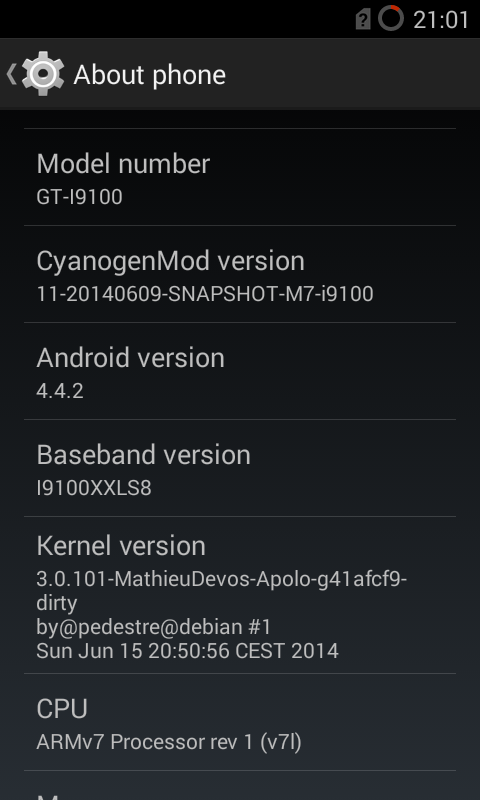
\includegraphics[width=0.5\textwidth]{figures/screenshot-kernel-i9100}
    \caption{Screenshot of ``About phone'' section of settings} 
    \label{fig:screenshot-kernel-i9100}
\end{figure}

\npar

Before we can move on to other subsections we have to note that this step is a very large step in the process and depending on the device, the support, the community, \ldots this can be a very lengthy process. We remark that this subsection, while now described simple, was quite a time-sink before we got to a working base kernel. This subsection is no longer as simple as just running the commands exactly as described on a website, so patches are needed, changes of files, and most of all: testing if the kernel will actually boot. If you find that the kernel gets stuck on boot, we note that Android does have any early boot warning system. However to access this system we need to set up a serial console with USB-to-UART converter. For this reason we strongly recommend to use matching code (kernel $\leftrightarrow$ ROM) which has been recently updated. 

\subsection{Android kernel with IRATI kernel code}

When we finally obtain the basic stable Android kernel with the code to build it, we can move towards adding the IRATI code to it. This subsection is only dedicated to the IRATI kernel code addition. Before we can implement the userspace, we first need a working kernel with all the correct kernel-specific code.
\npar
To add to this base kernel we use the git repository from IRATI over linux. Since Android is based on Linux we consider this to be a good starting point. The IRATI stack uses a base kernel and builds further on upon this. This means that when we create a patch that finds the differences between the base kernel and the IRATI kernel, we only have IRATI specific changes. This patch can then be applied to the base Android kernel in steps.
\npar
The patch will try to create new files when needed, change files or delete files which are no longer needed. However several issues arise here. In the current implementation of Linux, one can add system calls to the syscall table, called syscall\_32.tbl or syscall\_64.tbl depending on the architecture. These tables can be found in \emph{arch/x86/syscalls/}. However, this simply does not exist in our Android kernel. Not only does the file not exist, the map is simply non-existent. According to a guide\footnote{\url{http://www.techipost.com/2012/08/30/steps-of-adding-system-call-to-linux-kernel/}} we found on the Internet, we should be able to add these to unistd\_32.h. This is currently untested as we simply did not get this far yet because we have found issues with other files.
\npar
During the Make phase of the kernel we found ourselves stuck with the \emph{rmap.c} file. This calls for a hashtable function. This is where the first issue shows up. Hashtables are not implemented in Android, at least not in C. The solution to this was a fairly quick hack where we copied the hashtable.h file from a standard Linux kernel to the Android kernel. Now the function could be found, but we still had issues with one of the functions. The function: \emph{hlist\_for\_each\_entry\_safe} gives us the following error during compilation:
\\

\begin{lstlisting} 
net/rina/rds/rmap.c:87:68: error: macro "hlist_for_each_entry_safe" requires 5 arguments, but only 4 are given 
\end{lstlisting}

A quick glance at the code shows us that we are in fact passing 5 arguments to this function. Together with the previous issue of having difficulties of having to add system calls to the kernel, we are required to note that this might require an alternative approach. Since the user space implementation requires this kernelspace implementation to be functioning, the userspace subsection below has not been implemented in code as of yet. Due to the complexity of implementation that arose we are required to look for alternatives that will address both kernel- and userspace issues.

\subsection{Android compilation with glibc and IRATI userspace}

%First subsection about how to compile a base android kernel with glibc. Show steps taken to complete this process.

In this subsection we address the implementation of GlibC alongside Android. The reasons why we cannot stay with the same standard C library is fairly logic. Bionic, the C library for Android, does not provide full fledged support for \cpp, more on this can be read in the literature study~\ref{ssec:android-restrictions}. Simply said, if we want to install the userspace of IRATI, we will need access to a full C library. Several options are available here:

\begin{itemize}
	\item GNU C Library (glibc)
	\item dietlibc
	\item $\mu$clibc
	\item EGLIBC
\end{itemize}

We opted to for the most common library GlibC, because after further research we noted that this was the only one that had been implemented in Android. However it has never been done for the test devices, thus no previous experience could be relied upon. 
\\
After the implementation of the library we face another problem. Before the installation of the userspace can commence, we need some additional packages. The packages are freely available on Debian Wheezy systems. The packages are listed in the subsection, test bench irati (~\ref{ssec:test-bench-irati}). While these packages can be simply acquired from the source by running the standard ``apt-get install'' command (on Debian), this is unavailable in Android. The problem here is not that this command is OS-specific, it is that this command will also automatically check all dependencies for these packages. Furthermore is it possible that these packages do not support the ARM architecture, or are simply incompatible with the Android Operating System. 
\npar
Fixing this would require recompiling shell with GlibC so we would have a fully fledged shell with all commands. Next we would have to cross-compile every package and their dependencies separately. Then we would have to carefully install these packages on an alien system and hope that we would have the full functionality and commands available from these packages. This is clearly outside the scope of this Master's Thesis. Again, we need to look for an alternative. If this alternative is implementable within the timeframe of this Thesis is unknown.
\npar
A final remark about this userspace section of IRATI code. Currently the userspace section of IRATI provides RINA through the use of \cpp code. This can be seen in the figure~\ref{fig:userspacearch} below.  We note that these \cpp functions are mapped to JAVA with the use of SWIG. SWIG is an interface compiler which connects C and \cpp code to other languages, in our case: JAVA. 

\begin{figure}[H]
    \centering
    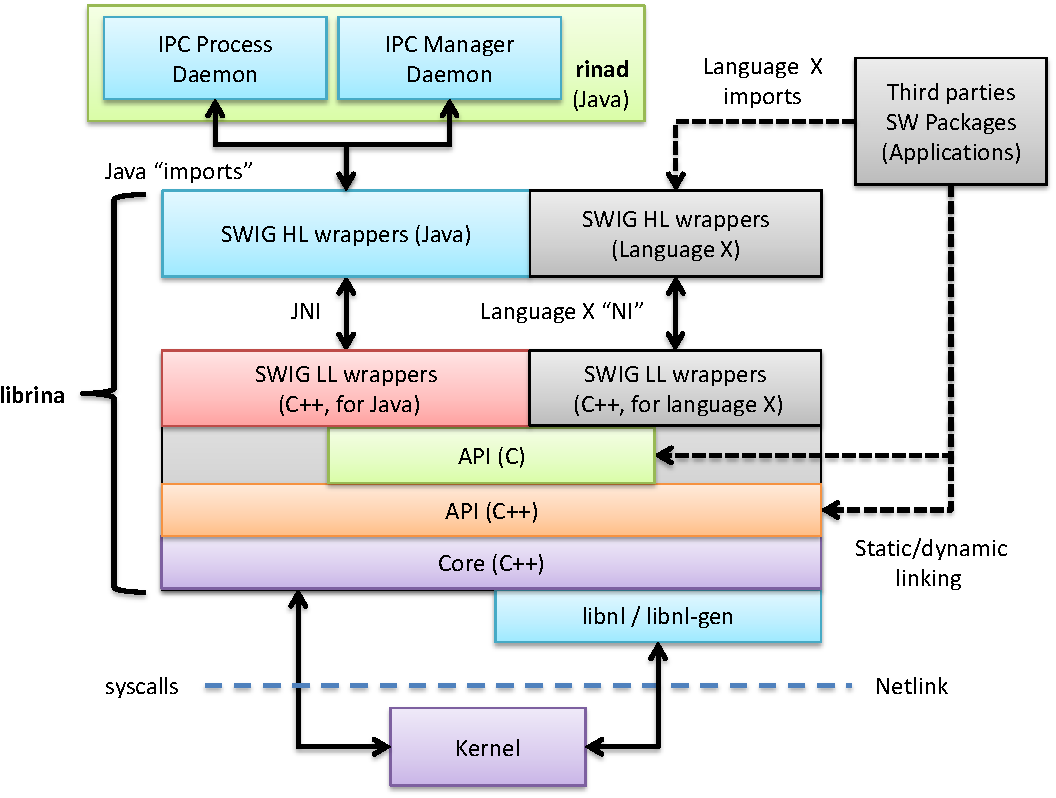
\includegraphics[width=1\textwidth]{figures/userspacearch}
    \caption{Overview of IRATI} 
    \label{fig:userspacearch}
\end{figure}

We see that the section of librina is mostly written in \cpp and then translated to Java functions through SWIG. This is the exact functionality that Android NDK also provides. It provides a environment that allows the developer to code in C or \cpp and translates this code to native libraries which can then be packed in \emph{.apk} files. These are Android specific files which represent programs. However, Android NDK comes with some limitations, as it is built for Android, it is specifically tailored to the Bionic library and does not support glibc. A solution for this is to use a different NDK, such as Crystax NDK\footnote{\url{https://www.crystax.net/en/android/ndk}}. These provide full support for \cpp and would thus perfectly fit for librina. If the kernel could be successfully implemented, the RINA userspace code that is written in \cpp (librina) should be imported in this NDK, adapted to the NDK and then produced as an .apk file. The rinad section (see figure~\ref{fig:userspacearch} above), is written in Java, thus can be copied to Android and be presented as a simple program. Of course, the librina can be imported as a native library then in one bigger program, which would also contain rinad. Given the current state of the IRATI project, this seems the most feasible solution towards implementation on Android.

\subsection{Android specific implementation}

%Specific implementation for the Galaxy S2, select stable kernel (cyanogenmod) and show changes made to add glibc and irati to it. Show if it works on the devices.

Following the previous subsections, this subsection is dedicated to an representation of the entire process. However, as we have noted we have encountered a plethora of difficulties in both kernelspace and userspace. This means that the actual implementation on the physical devices could not be realized and thus the test can not be completed. We do believe that while the original research question states: ``How to implement RINA on Android over WiFi'', we have proven that the WiFi aspect does not matter in this equation and that Android is a very strict platform. 
\npar
Because Android is such a specific platform we can see this research question in a different light. How to expand the IRATI codebase on different Linux-like Operating Systems, possibly with different architectures. In the final subsection of the implementation we address the alternatives that could prove to be helpful. Finally we attempt to show brief implementation processes that could be feasible for these alternatives, concerning RINA.

\subsection{Alternative implementation possibilities}

The final subsection is dedicated to alternatives of implementation. As we have shown during the previous (sub)sections, Android is very restricting. Within the current timeframe it is not possible to acquire a fully working RINA implementation with the IRATI codebase on Android. However we note that while Android is very restricting, other systems might be more viable for implementation of IRATI code. The goal is to stay on the same architecture, ARM. We see that different options become viable alternative paths. These options are:

\begin{itemize}
	\item Ubuntu Touch
	\item Debian next to Android
	\item Debian on Android
	\item Sailfish Operating System 
	\item More recent device
\end{itemize}

\npar

A quick glance over these options show that we are moving closer to less strict environments while still staying on the ARM architecture. While the most promising is most likely Ubuntu Touch, recently the entire development has been halted for the devices (i9100). This makes the Ubuntu Touch option a fairly unpredictable one as no backup or help can be found for the implementation of this. In its current form it is not possible to get the screen working and while Debian and Ubuntu are fairly similar, they are not exactly alike.
\npar
The second option of running Debian next to Android in its own space is a viable one, but has not been done for the device. This means that the same issues arise as the previous option: no help, no developing community, \ldots. While if it would be fairly easy to acquire this might be the best option, but as previously stated: this option falls short when paying respect to the limited timeframe. 
\npar
The third option, Debian on Android, might turn out to be the most interesting one. It has been done and can easily be implemented through Google Play Store. Several options are available such as:

\begin{itemize}
	\item Linux on Android
	\item Debian Kit
	\item Linux Deploy
	\item Complete Linux Installer
	\item \ldots
\end{itemize}

Given the limited timeframe we will attempt to test several of these devices and add our findings later. What we actually require from this: being able to construct our own kernel, if we get a base kernel and modify the IRATI kernel-specific code into this we can move towards the next step. Install this with Debian and attempt to install all the required userspace packages through ``apt-get install'', finally add swig through manual installation. This means that the packages will have to specifically run on ARM, or will have to be general and run on all architectures. Finally we have to note that this means that we are running Debian as a virtual machine on top of Android. This means that even if we can set up VLAN interfaces in the virtual machine, this does not mean that the Android device will use VLAN. More probably: we would have to set up RINA in such a way that we no longer care about VLAN tags, and instantly assume that all traffic is RINA traffic. Only if all these conditions are met will we be able to communicate between the two devices.
\npar
The second to last option that we will address here is the option of looking towards other operating systems that support ARM. Sailfish OS is such an operating system. It is built for ARM devices but ships with a fully fledged glibc library. Furthermore does it still support Android application through an adaptor layer. However, since no such device is physically available for this Master's Thesis we have to consider this option as an alternative, however not a viable alternative at this point of time.
\npar
The final option is simply to update the test devices. They run on kernel version 3.0.101, while newer devices easy run on 3.4.x. The newest devices will soon also start to be built for ARMv8 instead of ARMv7, which could open the doors further for technological improvements. Not only do new devices have more technological options, since they are newer most of these devices will have a bigger, more recent developing community, eager to get their hands on extra implementations. One of these implementations could be to acquire a working RINA on Android.
\npar
We can conclude that even with different alternatives we do not have one clear alternative that offers us the entire solution. While we have acquired plentiful knowledge about the subject and all relevant options, alternatives, \ldots. We have to consider the limited timeframe and scope of this Master's Thesis. The alternatives will be tested but we have to consider the downsides to each of these implementation alternatives.




\chapter{Conclusion}

%Conclusion of the master thesis, show followed path and give answer on the research question.

The final chapter presents the conclusion of the Master's Thesis. Here we show the path of operation we took starting from our introduction, through the literature study with the research question. Following this we conclude the specification and the implementation and finally we answer the research question in the final section.

\section{Plan of operation}

%Explain what was done first, how it was done, what the initial research question was. After this explain how the literature study affected the research question. Finally show the taken path of action with the implementation.

When we were originally presented with the Research question we were quite intrigued. A new architecture to replace the entire current Internet, that seemed like quite the task. Being part of this meant that we might be able to leave our mark on the pages of the Internet history. This is where we started this Master's Thesis, with the history of the Internet. It became quickly clear that the current version of the Internet had a lot of shortcomings, none of which could be addressed properly. A clear, new architecture was needed, RINA was born. A recursive architecture which reimplemented the same structure(s) over and over again, only changing their policy and scope. While RINA was purely theoretical, the IRATI project aimed to make a technical implementation at the lowest possible level for RINA. 
\npar
This is where the Master's Thesis is slotted in. After the research question we could fully launch our literature and technology study. This quickly brought us to an important milestone. A part of the research question, the wireless part, was unavailable in its current implementation. We had to drop this part from our implementation. We did provide a specification for the Shim DIF over Wireless. This specification provides enough information to the reader to implement a full wireless implementation of the IRATI code. Given the current Linux kernel code, this implementation can be seen as writing a driver for a network device. This was outside the scope of this Master's Thesis, thus we assumed the specification to be an adequate substitution for the lack of implementation over wireless medium. 
\npar
After providing the theoretical specification, we moved towards the implementation. Here we note that this implementation step was not initiated after the specification, but was already started during the preparation of the thesis. Initial base kernels were already constructed for both Linux and the Android devices (i9100 - Samsung Galaxy SII). Over the course of this Master's Thesis we have been acquiring information and learned how to practically apply this knowledge. However, we have to remark that even with the added knowledge, the amount of obstacles that presented themselves for this implementation piled up as well. Not only was finding a groundwork kernel for the devices a fairly specific and difficult task, which only proved to be successful after adding several manual patches to the code. We note that after the basic kernel we encountered many more problems, which, given the timeframe were simply not solvable. While we encountered these problems in both userspace and kernelspace, we opted to look for alternatives that could provide some relief to the implementation of the code. After careful research we have come to the conclusion that even these alternatives prove extremely difficult to implement given the current timespan of the thesis.

\section{Research question answer}

%Give an answer on the research question.

The research question states: \\
\begin{highlight}How to run RINA on Android over WiFi?\end{highlight}

\npar

We have to conclude that with the current implementation we are not able to run RINA on Android over WiFi. With the current Linux, and Linux-like, kernel the part about WiFi becomes irrelevant because the user is locked out of this process. A theoretical specification has been provided to answer the WiFi section. Furthermore have we shown extended research and implementation processes towards the Android part of the research question. However due to several, time-consuming difficulties, the implementation has proven to be a insufficient. The biggest issue we have here is a time issue. Given more time with added manpower and supplemented with additional knowledge, this implementation is feasible. Further research is required to acquire a working implementation of RINA on Android. 



\newpage								% Used to input empty page
\thispagestyle{empty}
\mbox{}

\appendix
\appendixpage

\chapter*{Appendix A: Emailconversation Linux Wireless mailing list}
\label{chap:app-a}

\fbox{\includegraphics[page=3,scale=0.6]{emailconvo.pdf}}
%\includepdf[pages={2-},scale=0.8]{emailconvo.pdf}
\chapter*{Appendix B: Construction of kernels guide}
\label{chap:app-b}


This guide stipulates how to create kernels for Linux, Android in general and specificcaly to the Samsung Galaxy SII device (i9100). We assume the person operating these systems to be utilizing a Debian or Debian-like system. Other systems might require different commands. 

\section*{Kernel compilation for linux}

First, lets get a kernel from \url{http://www.kernel.org} we recommend just getting a long term kernel that is based on your current kernel. For this guide we'll be using the \engels{3.2.49 linux kernel}\footnote{\url{https://www.kernel.org/pub/linux/kernel/v3.x/linux-3.2.49.tar.xz}}.

\npar

Now you'll want to extract 
\begin{quote} \begin{verbatim}tar -xvf linux-3.2.49.tar.xz \end{verbatim} \end{quote} 
and move to the directory of this kernel.
\begin{quote} \begin{verbatim}cd linux-3.2.49/ \end{verbatim} \end{quote}

\npar

Before we go any further we'll need some packages to ensure a proper build and help us down the road. To get these packages run:

\begin{quote} \begin{verbatim}sudo apt-get install libncurses5-dev gcc make git exuberant-ctags \end{verbatim} \end{quote}

Note that for pure kernel building you can follow the guide from KernelNewbies\footnote{\url{http://kernelnewbies.org/KernelBuild}}, this section will follow this guide quite a bit but will show where you can make changes.

\npar 

If you do not wish to download a .tar you can opt to get the code directly from the git as shown on KernelNewbies with the following command:

\begin{quote} \begin{verbatim}git clone link.git && cd map  \end{verbatim} \end{quote}

After this you might still need to check out to the correct branch. To list them run:

\begin{quote} \begin{verbatim}git branch -a \end{verbatim} \end{quote}

Check out the branch you want (stable, longterm, ...) with:

\begin{quote} \begin{verbatim}git checkout -t origin/branchname \end{verbatim} \end{quote}

Now we need a configure file for this kernel, several options are available here.

\subsection*{Copy current configure file}

This is most likely the simplest and fastest way to set up your config file. Simply copy your current config file and place it in the kernel folder (named \engels{.config} - this means it's an invisible file). This can be easily done with the follow command:

\begin{quote} \begin{verbatim}cp /boot/config-`uname -r`* .config \end{verbatim} \end{quote}

Note that this command will have to be run from inside the kernel directory. The part \engels{uname -r} basically prints your current kernel version thus it will select the config for your current active kernel (important if you have multiple kernels).

\subsection*{Making default configuration}

This is the very default configuration. If you run this you and instantly try to compile your kernel you will get a huge number of questions trying to figure out how to set up your kernel. This can take a while and could leave you without some important options (it's easy to miss them). Hence why we recommend to copy your own config and make changes to it (see subsection menuconfig below). If you want to create a default config, just run this code from the kernel directory:

\begin{quote} \begin{verbatim}make defconfig \end{verbatim} \end{quote}

\subsection*{Making non-default configuration}

Some kernels provide more base configuration files, you can find these in \engels{arch/your\_architecture/configs}. If you are unsure what your architecture is, just run

\begin{quote} \begin{verbatim}uname -m \end{verbatim} \end{quote}

Lets say you have a config file name x86\_64 in there that is a config file. To prepare your build with this configuration file, just run 

\begin{quote} \begin{verbatim}make x86_64 \end{verbatim} \end{quote}

from your kernel base directory.

\subsection*{Change configuration file}

Once you have your configuration file (through copy or make defconfig) you can edit this through a simple visual editor with the following commands:

\begin{quote} \begin{verbatim}make menuconfig \end{verbatim} \end{quote}

or 

\begin{quote} \begin{verbatim}make nconfig \end{verbatim} \end{quote}

\subsection*{Kernelcompilation}

The actual kernel compilation is done by running the following command from your kernel base directory:

\begin{quote} \begin{verbatim}make \end{verbatim} \end{quote}

This can take a while and if you have a multicore processor you can advantage of this by adding an option to this make. The command becomes:

\begin{quote} \begin{verbatim}make -j`nproc` \end{verbatim} \end{quote}

Nproc will return the number of cpu cures thus this will run make with just as much threads as you have cpu cores.

\section*{Kernel compilation for android}

For android a small part is different, but it's the general idea that stays the same.

\subsection*{Toolchain}

Android needs to be build with a custom gcc toolchain. This toolchain can be found at: \url{https://github.com/mathieudevos/arm-eabi-4.6}. With git this becomes

\begin{quote} \begin{verbatim}git clone https://github.com/mathieudevos/arm-eabi-4.6.git \end{verbatim} \end{quote}

Note that you should \textbf{NOT} be in your kernel directory, it is recommended that you run this git command in the parent folder of the kernel. This would end up with one folder named linux-3.2.49 and one named arm-eabi-4.6.

\npar

Older toolchains might not work on your system as 4.6 is the first one to be written for 64bit operating systems (note that this entire process is written for 64bit). Once you have the toolchain we now need to point the Makefile to this toolchain.

\subsection*{Initramfs for android}

Since this can not be automatically copied from your current kernel you need to specify your own initramfs. While you can build your own initramfs with following script: \engels{kernel/scripts/gen\_initramfs\_list.sh}, we do not recommend it as you need a very specific set of parameters for this. 

\npar

If you are only building your kernel for the sake of kernel modules (thus just matching version) you can use the default initramfs file by just running

\begin{quote} \begin{verbatim}./gen_initramfs_list.sh -u 0 -g 0 -d > default_initramfs.list \end{verbatim} \end{quote}



\npar

For a normal kernel build that you intend to install we recommend you ``steal'' an initramfs file from an existing kernel. For the I9100 device we will provide our own initramfs that should work, it can be found here: \url{https://github.com/mathieudevos/android_kernel_samsung_smdk4210/blob/cm-10.1/usr/galaxys2_initramfs.list}. 

\npar

After you have acquired your initramfs file you just need to make your kernel point towards it, this is done in the \engels{.config} file, change the follow field:

\begin{quote} \begin{verbatim}CONFIG_INITRAMFS_SOURCE="./usr/galaxys2_initramfs.list" \end{verbatim} \end{quote}

\subsection*{Kernel build preparation}

Open the \engels{Makefile} in your kernel folder with a text editor. Find and change to the following data fields:

\begin{quote} \begin{verbatim}ARCH ?= arm
CROSS_COMPILE ?= ../arm-eabi-4.6/bin/arm-eabi- \end{verbatim} \end{quote}

\npar

After this is done you can open your \engels{.config} file and change your 

\begin{quote} \begin{verbatim}CONFIG_LOCALVERSION="" \end{verbatim} \end{quote}

If you have a very similar kernel to the one you are currently running and only wish to use this kernel for building kernel modules you must make sure this name reflects your kernel name. The versions should match (see on top of Makefile) and also the localversion should match. 
\npar
Sometimes however, it is easier to build a kernel from scratch and install said kernel and only after that is done start building your kernel modules on this kernel. This will insure good integration between your kernel modules and your kernel.


\section*{Kernel installation for linux}

The linux kernel that you just compiled can easily be installed into your current system by running following commands from the base kernel directory:

\begin{quote} \begin{verbatim}sudo make modules_install install \end{verbatim} \end{quote}

This will install your kernel to the \engels{/boot/} folder, install your modules (the ones shipped with your kernel, we will make our own) and update your grub bootloader. To use this command you do need an installkernel script, which grubby provides.

\npar

If you want to be sure your grub bootloader will present you with the option of choosing your kernel on boot you should make a few modifications in the grub file. This file can be found at \engels{/etc/default/grub}. To ensure that you are always presented with the option of choosing your kernel, delete the following line:

\begin{quote} \begin{verbatim}GRUB_HIDDEN_TIMEOUT_QUIET \end{verbatim} \end{quote}

If you want you can still change the timeout timer so you have a bit more time to choose your kernel. Just edit:

\begin{quote} \begin{verbatim}GRUB_DEFAULT timeout \end{verbatim} \end{quote}

After you modified this file, just finish with the command:

\begin{quote} \begin{verbatim}sudo update-grub2 \end{verbatim} \end{quote}

This concludes the Linux kernel building and installation. You should now be able to build your own linux kernel and boot into it.

\section*{Kernel installation for android}

Android is quite a bit harder to install your own kernel. After you are done with building your kernel with the toolchain you will find a zImage (or similar name) in your \engels{kernel/arch/arm/boot} folder. This is the image that we want to flash onto our device.

\npar

Depending on your device this is done after you unlocked your bootloader (general setup) or for instance with a specific tool (heimdall) for older devices like \engels{Samsung Galaxy S2 - I9100}. After you have your zImage ready we now need to overwrite your old zImage. \\

\begin{warning}
\textbf{unlocking your bootloader and/or installing new kernels can void your warranty, we cannot be help responsible for any damages caused by following this guide}
\end{warning}

\subsection*{General install on newer devices}

After you have unlocked your phone (google this) you should install android sdk which should give you access to fastboot. You can confirm this by plugging your device in and running

\begin{quote} \begin{verbatim}fastboot devices \end{verbatim} \end{quote}

For this command to work you have to be in fastboot mode, this is mostly done by a hardware key combination on boot, google this for your phone. This command should show your device in the terminal window. Once you have this, lets move to our zImage folder and try to boot with this kernel (but not flash it).

\begin{quote} \begin{verbatim}fastboot boot zImage \end{verbatim} \end{quote}

If your phone boots properly into your new kernel and you can check this within settings that this is actually your kernel, you can repeat the process but now flash your kernel.

\begin{quote} \begin{verbatim}fastboot flash zimage zImage \end{verbatim} \end{quote}

This concludes installing your zImage through fastboot.

\subsection*{Specific installation on galaxy S2}

If you do not have a galaxy S2 you should skip this part as it uses a custom program that only works for this device.

\npar

Boot your phone into download mode (press volume down, power and menu for 10 seconds). Once you have your phone in this mode, go to download mode. From this mode run the heimdall command with:

\begin{quote} \begin{verbatim}heimdall print-pit \end{verbatim} \end{quote}

This should return the partition points with the images attatched to them. We're looking for the zImage here, it'll be called \engels{kernel} or \engels{KERNEL}, this is important because it's case sensitive. Once you have this information, get ready to flash your zImage on the device with:

\begin{quote} \begin{verbatim}heimdall flash --KERNEL zImage \end{verbatim} \end{quote}

After this your phone should reboot with your new kernel on it.



%\chapter{Background study 802.11}

\section{802.11 header} %changed to header

%\begin{table}[h]
	%	\centering
		%\noindent
		%\small
	%	\begin{tabulary}{1\textwidth}{|C|C|C|C|C|C|C|C|C|C|C|C|}
	%	
	%		\hline
	%			\mc{} & Frame Control & Duration / ID & Address 1 & Address 2 & Address 3 & Sequence Control & Address 4 & QoS Control & HT Control & Frame Body & FCS \\ \hline
	%			\mc{Bytes} & \mc{2} & \mc{2} & \mc{6} & \mc{6} & \mc{6} & \mc{2} & \mc{6} & \mc{2} & \mc{4} & \mc{0-7951} & \mc{4} \\
	%	\end{tabulary}
%		\caption{802.11 MAC frame format}
%\end{table}

\begin{figure}[H]
    \centering
    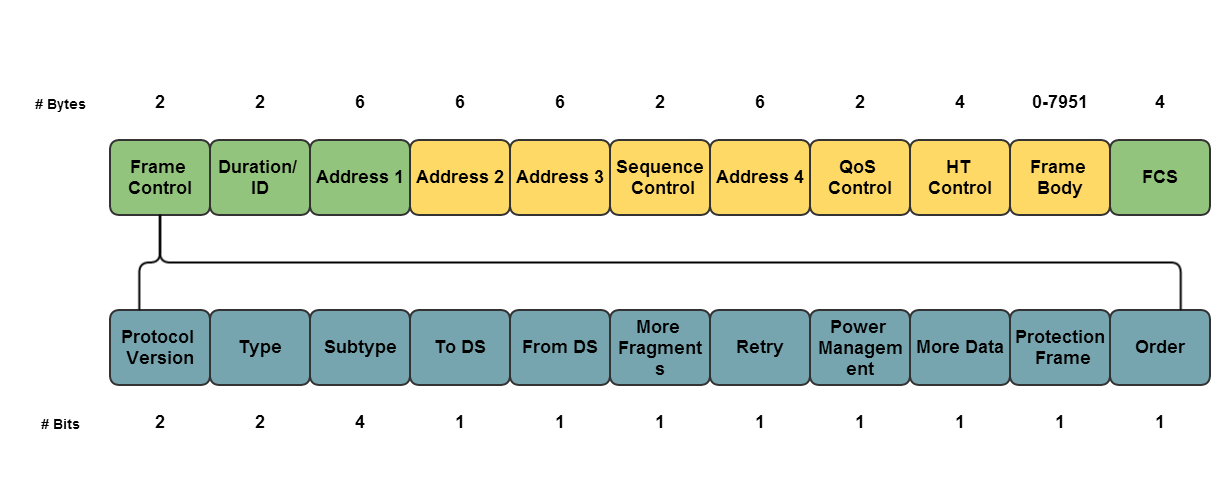
\includegraphics[width=1\textwidth]{figures/80211macframe}
    \caption{802.11 MAC frame} 
    \label{fig:80211macframe_bg}
\end{figure}


\subsection{Frame Control}

In this section a closer look will be taken at the Frame Control. This part is a requirement in every 802.11 MAC frame and will be carefully analyzed. 

\subsubsection{Protocol Version}

This first field consists of 2 bits and is currently always 00. The field is fully reserved for future revisions of the 802.11 header. This field will always stay 00 in the current version of the SHIM DIF.

\subsubsection{Type \& Subtype}

Two fields that consist of 2 and 4 bits. The combination of these two fields determines the function of the current frame. Currently 3 different types are used as type field, these are: 
\begin{itemize}
	\item Management
	\item Control
	\item Data
\end{itemize}

Since these fields are used to set up communication between two devices these fields won't be touched on in the SHIM DIF. Further information on these fields can be found in the IEEE Std. 2012~\citep{ieee80211std}

\subsubsection{To DS \& From DS}

The next two fields are fairly self-explanatory. They decide whether a packet is traveling from or towards a Distribution System (DS). When both of these fields are set to 0 it implies that a frame is traveling straight from one STA to another STA without going to a DS first. Both fields on value 1 means that we are using this in mesh mode and the 4 addresses will be used. Since this SHIM DIF should only providing base function for 802.11 this will not be handled further.

\subsubsection{More Fragments}

This one bit field is set to 1 when either data or management frames have more fragments. In all other cases it should be 0.

\subsubsection{Retry}

A one bit field limited to data or management frames. It is set to 1 when this frame is a retransmission, in all other cases it is set to 0.

\subsubsection{Power Management}

This one bit field's value is heavily reliant on the entire frame. For this limited use SHIM DIF the use of this frame should be copied from the 802.11 standard~\citep{ieee80211std}.

\subsubsection{More Data}

Another one bit field with a specific purpose that will be copied from the standard. This field provides information about following frames that are buffered at the AP for this specific STA.

\subsubsection{Protection Frame}

The second to last field in the Frame Control field is like many other fields a 1 bit field. This bit contains information about the Frame Body. When this Frame Body contains information that has been encrypted this field is set to 1. This is however only the case in specific cases and should be carefully analyzed from the standard. An example here is that this field can never be set to 1 when the Frame Body does not contain any data at all.

\subsubsection{Order}

The final bit in the Frame Control field provides two purposes. It can be set to one in either non-QoS frame or in QoS frames. In both the 1 value provides a different use for the system. Since this also has no further use for the SHIM DIF it will not be handled in detail.

\subsection{Duration / ID}

After the Frame Control field we have the second required field to make a valid 802.11 frame. This is the Duration or ID frame. The frame is 2 bytes (16 bits) large and can be used in various ways. This field is dependent on the type and subtype field earlier mentioned in the Frame Control field. It provides information for the total duration of the frame or provides an ID that can be used to identify and order the frame in it's rightful order. 

\subsection{Address 1, 2, 3 \& 4}

These 4 address fields all use the same type of address fields used in other Ethernet MAC frames. They consist of 6 bytes (48 bits) each and only address 1 most be filled in to complete a valid frame. The addresses can be used for following purposes:

\begin{description}
	\item[BSSID] Basis Service Set Identifier 
	\item[SA] Source Address
	\item[DA] Destination Address
	\item[TA] Transmitting STA Address
	\item[RA] Receiving STA Address
\end{description}

These fields are to be used as the points of attachment MAC addresses of the underlying interfaces. The shim DIF is bound to these interfaces through this address. 

\subsection{Sequence Control}

A 2 byte field that is split up in 2 subfields. Note that this field is not present in control frames, only in data and management ones. The first subfield is the fragment number and is 4 bits long. This subfield tells the fragment number of the frame, starting at 0 for the very first piece and incrementing by 1 step for every consequent fragment. The second subfield is 12 bits long and is the sequence number subfield. This number is the order of the frames and provides information towards the system about the order of frames.

\subsection{QoS Control}


This field provides information about QoS (Quality of Service) settings the frame currently provides. The 16 bit value is dependent on the type, subtype and the transmitting STA of the frame. QoS Control field is needed when the QoS bit in the subtype of a frame is set to 1. The field often contains information about Traffic Identifiers (TID), ACK policy, EOSP, \ldots. A closer look in at these different fields can be taken in the 802.11 standard document~\citep{ieee80211std} (p389). 

\subsection{HT Control}

The final field before the actual frame body is a 4 byte field. The field contains information about the High Throughput of the frame. It is present in Control Wrapper frames and QoS data frames. Since this has little use in RINA it will left as it is and copied exactly from the current standard~\citep{ieee80211std}.

\subsection{Frame Body}

This field is between 0 and 7951 bytes long and contains the actual body of the frame. This will contain further DIFs and ultimately the actual data is should be transferred. Notice that for some frames this can actually be 0, this implies it can be an optional field.

\subsection{FCS}

Final field of the 802.11 frame is a 4byte long Frame Control Sequence. It contains a 32 bit CRC calculated over the entire MAC frame, including the body. The use of this field is to detect errors in the entire frame. It should be copied exactly for the SHIM DIF usage.


% De appendices:
%%%\appendix



% De bibliografie en de index
\backmatter

\bibliography{bibliography_md}

%\begin{appendices}
%\appendix
%%%\appendixpage
%\renewcommand{\section}{\Alph{section}}
%\section{Email conversation Linux Wireless Mailinglist}
%\label{chap:emailconvo}
%\begin{figure}[H]
%    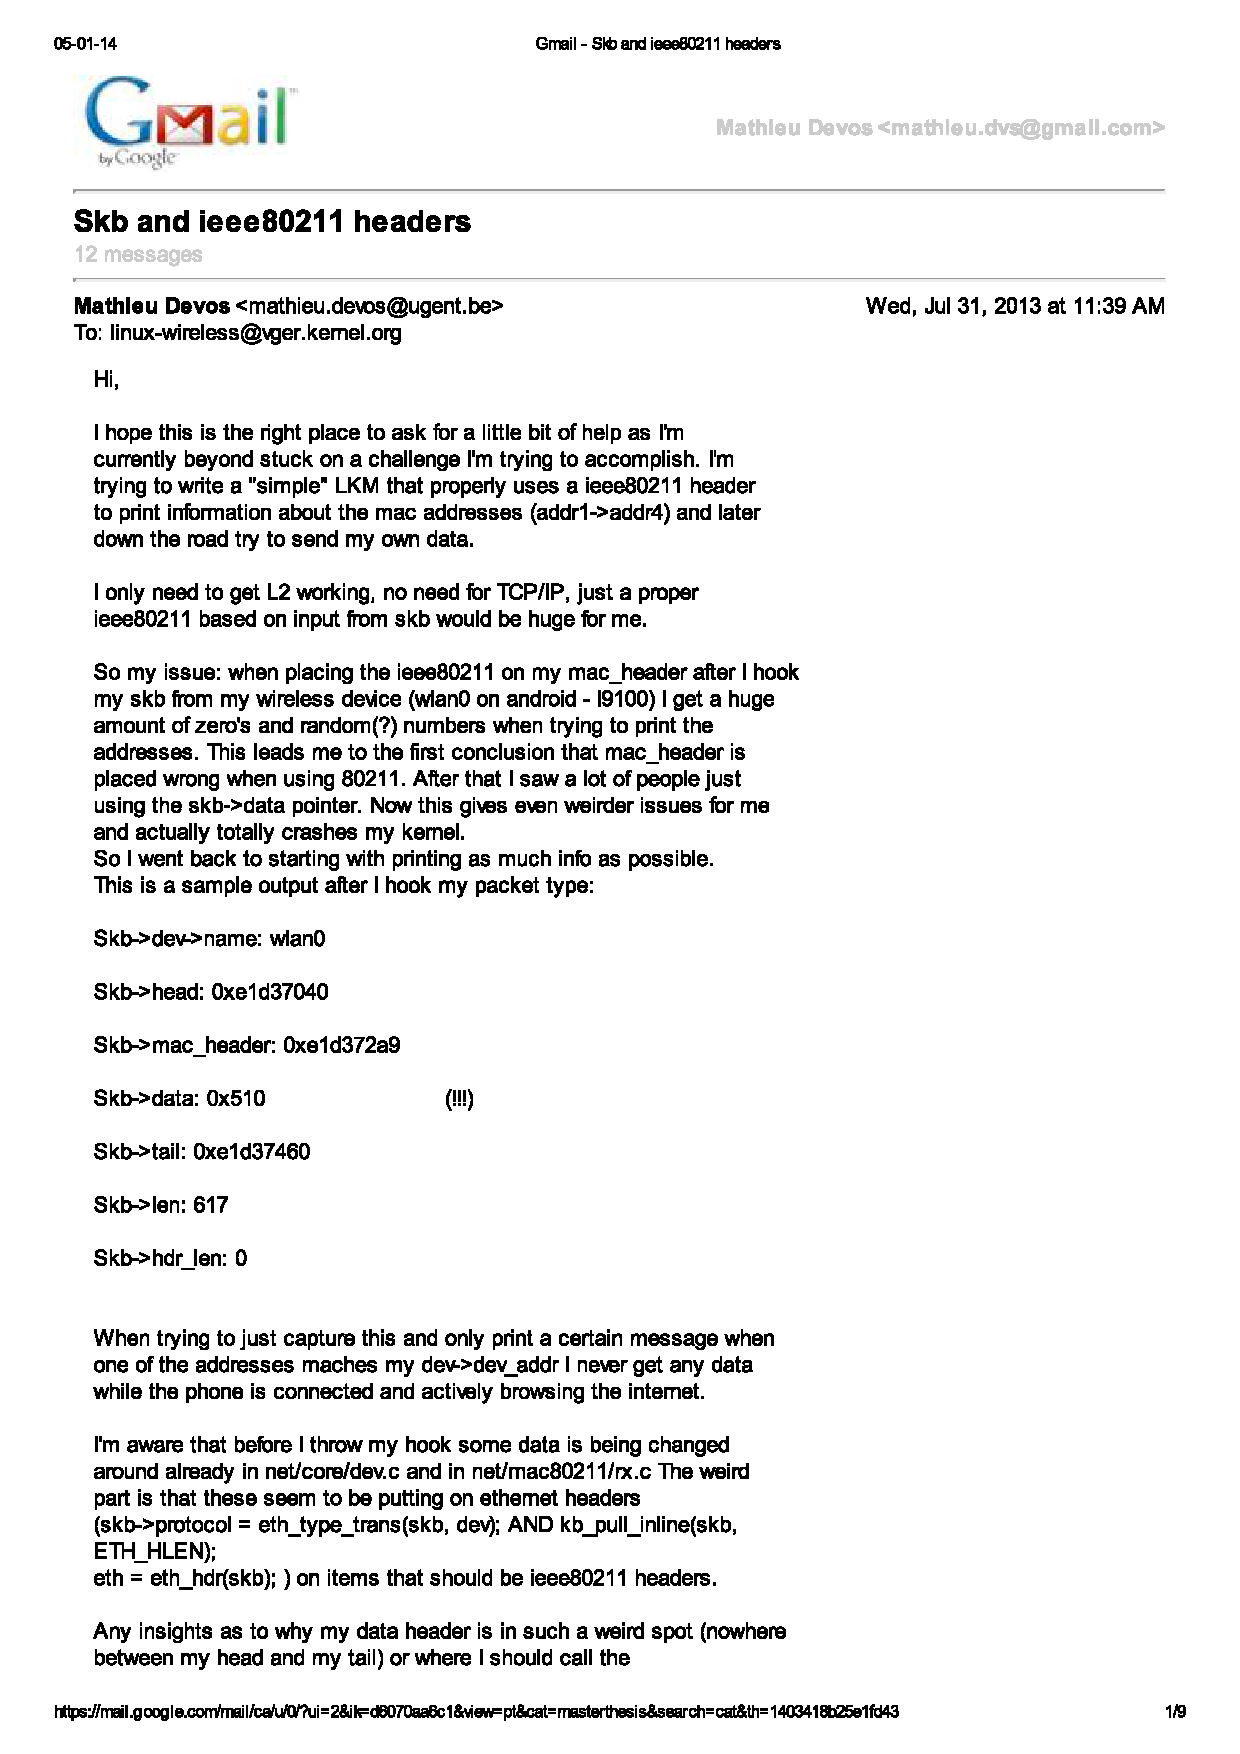
\includegraphics[scale=0.7]{emailconvo}
%\end{figure}
%\includepdf[pages=3,scale=0.8]{emailconvo.pdf}


%\section{Proof of concept over WiFi logs}
%\label{chap:poc-wifi-logs}
%\subsection{Modprobe shim-eth-vlan}

\lstinputlisting{log-modprobe-shim-eth-vlan.txt}

\subsection{Modprobe normal-ipcp}

\lstinputlisting{log-modprobe-normal-ipcp.txt}

\subsection{ipcmanager}

\lstinputlisting{log-ipcmanager.txt}
%\end{appendices}

%\printindex                             % Om de index af te printen, niet bij een thesis.

\newpage								% Used to input empty page
\thispagestyle{empty}
\mbox{}
\newpage								% Used to input empty page
\thispagestyle{empty}
\mbox{}



\end{document}



